\chapter{Noțiuni teoretice}

\section{Procesare de imagine}

\subsection*{Ce este imaginea digitală și procesarea de imagine?}

O imagine poate fi definită ca o funcție bidimensională, f$(x,y)$, unde x și y sunt coordonate spațiale, iar amplitudinea lui f la orice pereche de coordonate $(x, y)$ este numită intensitatea sau nivelul de gri al imaginii în acel punct. Când x, y și valorile intensității lui f sunt finite și discrete, imaginea se numește imagine digitală. Procesarea imaginii digitale se referă la procesarea imaginilor digitale cu ajutorul unui computer digital. O imagine digitală este compusă dintr-un număr finit de elemente, fiecare având o locație și o valoare specifică, numite pixeli.

Viziunea este cel mai avansat simț al nostru, astfel încât imaginile joacă un rol esențial în percepția umană. Spre deosebire de oameni, care sunt limitați la spectrul vizual al radiațiilor electromagnetice, mașinile de imagistică acoperă aproape întregul spectru electromagnetic, de la raze gamma la unde radio. Acestea pot opera pe imagini generate de surse neobișnuite pentru oameni, cum ar fi ultrasunetele, microscopie electronică și imagini generate de computer.

Nu există un acord general privind granițele dintre procesarea imaginii, analiza imaginii și viziunea computerizată. Uneori, procesarea imaginii este definită ca o disciplină în care atât intrarea, cât și ieșirea sunt imagini. Aceasta poate fi o definiție limitativă. Pe de altă parte, viziunea computerizată are ca scop imitarea vederii umane, inclusiv învățarea și luarea deciziilor pe baza inputurilor vizuale, fiind o ramură a inteligenței artificiale.

Un exemplu de procesare a imaginii digitale este analiza automată a textului, care include achiziția imaginii, preprocesarea, extragerea și recunoașterea caracterelor individuale. Înțelegerea conținutului paginii poate fi considerată analiză a imaginii sau chiar viziune computerizată, în funcție de complexitate.

\subsection*{Spații de culoare}

În procesarea imaginilor, spațiile de culoare sunt modalități de a reprezenta culorile în modele numerice care facilitează manipularea și analiza imaginilor. Cele mai comune spații de culoare utilizate sunt Grayscale, RGB și HSV.

Grayscale (tonuri de gri) este un spațiu de culoare în care fiecare pixel este reprezentat de o singură valoare care indică intensitatea luminii. Valorile sunt de obicei cuprinse între 0 (negru) și 255 (alb) pentru imagini pe 8 biți. Conversia unei imagini color într-o imagine grayscale se face prin combinarea componentelor de culoare ale fiecărui pixel într-o singură valoare de luminanță.

\begin{figure}[htbp]
    \centering
    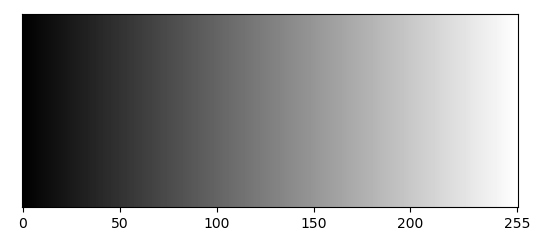
\includegraphics[width=0.5\textwidth]{images/grayscale.jpg}
    \caption{Gradientul Grayscale \cite{wiki_grayscale}}
\end{figure}
\FloatBarrier

RGB (Red, Green, Blue) este un spațiu de culoare aditiv în care orice culoare poate fi creată prin combinarea celor trei culori primare: roșu, verde și albastru. Fiecare componentă are o valoare între 0 și 255 într-o imagine pe 8 biți.

\begin{figure}[htbp]
    \centering
    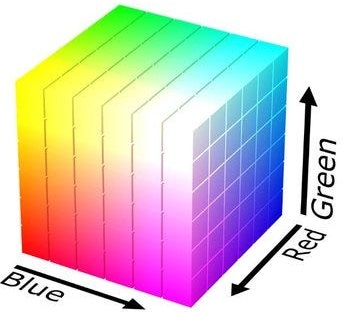
\includegraphics[width=0.5\textwidth]{images/RGB.jpg}
    \caption{Cubul RGB \cite{wiki_rgb}}
\end{figure}
\FloatBarrier

HSV (Hue, Saturation, Value) este un spațiu de culoare care reprezintă culoarea într-un mod mai intuitiv pentru percepția umană. Cele trei componente sunt:
\begin{itemize}
    \item \textbf{Hue (nuanță)}: descrie tipul de culoare și este măsurat în grade de la 0 la 360.
    \item \textbf{Saturation (saturație)}: descrie intensitatea culorii și variază de la 0 (gri) la 1 (culoare pură).
    \item \textbf{Value (valoare)}: descrie luminozitatea culorii și variază de la 0 (negru) la 1 (alb complet).
\end{itemize}

\begin{figure}[htbp]
    \centering
    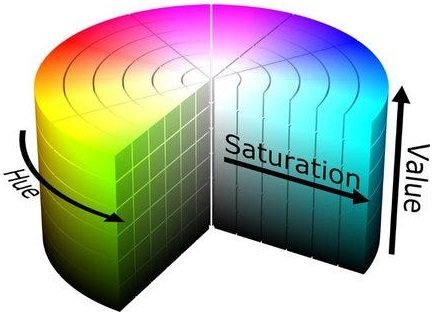
\includegraphics[width=0.5\textwidth]{images/HSV.jpg}
    \caption{Cilindrul HSV \cite{wiki_hsv}}
\end{figure}
\FloatBarrier

Conversia între diferite spații de culoare este adesea necesară în procesarea imaginilor pentru a facilita anumite operații. Aceste conversii permit adaptarea și prelucrarea imaginilor în funcție de cerințele specifice ale aplicațiilor, fie că este vorba de îmbunătățirea contrastului, identificarea obiectelor sau alte tehnici de analiză. Iată câteva formule de bază pentru conversie:
\begin{enumerate}
    \item \textbf{Conversia RGB la Grayscale}:
          \[
              Y = 0.299 \cdot R + 0.587 \cdot G + 0.114 \cdot B
          \]
          Această formulă folosește o combinație ponderată a componentelor roșu, verde și albastru pentru a calcula luminanța, rezultând o imagine în tonuri de gri care păstrează percepția de lumină a imaginii originale.

    \item \textbf{Conversia RGB la HSV}:
          \[
              C_{\max} = \max(R, G, B)
          \]
          \[
              C_{\min} = \min(R, G, B)
          \]
          \[
              \Delta = C_{\max} - C_{\min}
          \]

          \[
              H = \begin{cases}
                  0                                                               & \text{dacă } \Delta = 0   \\
                  60^\circ \times \frac{G - B}{\Delta} + 360^\circ \mod 360^\circ & \text{dacă } C_{\max} = R \\
                  60^\circ \times \frac{B - R}{\Delta} + 120^\circ                & \text{dacă } C_{\max} = G \\
                  60^\circ \times \frac{R - G}{\Delta} + 240^\circ                & \text{dacă } C_{\max} = B
              \end{cases}
          \]

          \[
              S = \begin{cases}
                  0                       & \text{dacă } C_{\max} = 0 \\
                  \frac{\Delta}{C_{\max}} & \text{altfel}
              \end{cases}
          \]

          \[
              V = C_{\max}
          \]

          Conversia RGB la HSV este utilă deoarece spațiul HSV este mai intuitiv pentru percepția umană a culorilor, facilitând operații cum ar fi ajustarea saturației sau a nuanței fără a afecta celelalte componente de culoare.

    \item \textbf{Conversia HSV la RGB}:
          \[
              C = V \times S
          \]
          \[
              X = C \times (1 - \left| \left(\frac{H}{60^\circ} \mod 2 \right) - 1 \right|)
          \]
          \[
              m = V - C
          \]

          \[
              (R, G, B) = \begin{cases}
                  (C+m, X+m, m) & \text{dacă } 0 \leq H < 60^\circ          \\
                  (X+m, C+m, m) & \text{dacă } 60^\circ \leq H < 120^\circ  \\
                  (m, C+m, X+m) & \text{dacă } 120^\circ \leq H < 180^\circ \\
                  (m, X+m, C+m) & \text{dacă } 180^\circ \leq H < 240^\circ \\
                  (X+m, m, C+m) & \text{dacă } 240^\circ \leq H < 300^\circ \\
                  (C+m, m, X+m) & \text{dacă } 300^\circ \leq H < 360^\circ
              \end{cases}
          \]

          Această conversie permite transformarea din spațiul de culoare HSV în RGB, ceea ce este util pentru afișarea imaginilor după ce au fost manipulate în spațiul HSV. Conversiile între aceste spații de culoare permit efectuarea de prelucrări complexe pe imagini, cum ar fi filtrarea bazată pe nuanță sau saturație, care sunt greu de realizat direct în spațiul RGB.
\end{enumerate}

\subsection*{Coordonatele}

Coordonatele sunt utilizate pentru a descrie poziția unui punct într-un spațiu bidimensional. Un punct este definit printr-o pereche ordonată de valori care indică poziția sa pe cele două axe ale sistemului de coordonate.

Considerăm un punct \( P \):
\[
    P = (x, y)
\]
unde \( x \) reprezintă coordonata pe axa orizontală, iar \( y \) coordonata pe axa verticală. Fiecare pereche \((x, y)\) identifică un punct unic în spațiu.

Pentru o mulțime de puncte \( \mathcal{R} \), este adesea util să definim o poziție medie a acestora. Această poziție se numește centroid și reprezintă centrul geometric al mulțimii de puncte.

Coordonatele centroidului sunt:
\[
    \bar{x} = \frac{1}{N} \sum_{(x,y) \in \mathcal{R}} x, \quad
    \bar{y} = \frac{1}{N} \sum_{(x,y) \in \mathcal{R}} y
\]
unde \( N \) este numărul total de puncte din mulțime. Centroidul este astfel:
\[
    C = (\bar{x}, \bar{y})
\]

În anumite situații, coordonatele sunt transformate într-un interval standardizat pentru a elimina dependența de scară. Această operație se numește normalizare.

Considerând un domeniu de dimensiuni \( W \times H \), coordonatele normalizate ale unui punct \( (x, y) \) sunt:
\[
    x' = \frac{x}{W}, \quad y' = \frac{y}{H}
\]

Valorile normalizate aparțin intervalului:
\[
    x', y' \in [0, 1]
\]

Normalizarea permite reprezentarea coordonatelor într-o formă independentă de dimensiunea absolută a domeniului și facilitează compararea punctelor definite în sisteme diferite.

\subsection*{Histograma}

Să notăm cu $r_k$, pentru $k = 0, 1, 2, \ldots, L-1$, intensitățile unei imagini digitale de nivel $L$, $f(x, y)$. Histograma ne-normalizată a lui $f$ este definită ca:
\[
    h(r_k) = n_k \quad \text{pentru } k = 0, 1, 2, \ldots, L-1
\]
unde $n_k$ este numărul de pixeli din $f$ cu intensitatea $r_k$, iar subdiviziunile scalei de intensitate sunt numite \textit{bin-uri de histogramă}. În mod similar, histograma normalizată a lui $f$ este definită ca:
\[
    p(r_k) = \frac{h(r_k)}{MN} = \frac{n_k}{MN}
\]
unde, ca de obicei, $M$ și $N$ sunt numărul de rânduri și coloane ale imaginii, respectiv. În general, lucrăm cu histograme normalizate, la care ne referim simplu ca histogramă sau histograme de imagine. Suma valorilor $p(r_k)$ pentru toate valorile lui $k$ este întotdeauna 1. Componentele $p(r_k)$ sunt estimări ale probabilităților de apariție a nivelurilor de intensitate într-o imagine.

Pe baza histogramei normalizate se poate defini și funcția de distribuție cumulativă:
\[
    P(r_k) = \sum_{j=0}^{k} p(r_j)
\]
care reprezintă probabilitatea ca intensitatea să fie mai mică sau egală cu $r_k$. Această funcție este utilă pentru determinarea percentililor. De exemplu, percentila $q$ este valoarea $r_k$ pentru care:
\[
    P(r_k) \geq q
\]
unde $q \in [0,1]$. Percentilii sunt utilizați frecvent pentru analiza distribuției intensităților, eliminarea valorilor extreme sau ajustarea contrastului prin tăierea valorilor din cozi (de exemplu, percentilele 5\% și 95\%).

Forma histogramei este legată de apariția imaginii. De exemplu, presupunem imagini cu patru caracteristici de bază ale intensității: întunecată, luminoasă, contrast scăzut și contrast ridicat. Într-o imagine întunecată, cele mai populate bin-uri ale histogramei sunt concentrate la capătul inferior al scalei de intensitate. Similar, majoritatea pixelilor luminoși sunt concentrați spre capătul superior al scalei de intensitate. O imagine cu contrast scăzut are o histogramă îngustă situată de obicei în jurul mijlocului scalei de intensitate.

Într-o imagine cu contrast ridicat, componentele histogramei acoperă un interval larg al scalei de intensitate, iar distribuția pixelilor nu este prea departe de uniformă. Utilizarea percentililor permite evaluarea mai robustă a acestui interval, ignorând valorile extreme care pot distorsiona percepția contrastului. Intuitiv, o imagine ale cărei pixeli ocupă o mare parte din intervalul de intensitate și sunt distribuiți relativ uniform va avea un aspect bogat în detalii și un interval dinamic ridicat.

\subsection*{Decupare și redimensionare}

Decuparea (crop) este o operațiune esențială în prelucrarea imaginilor care presupune selecționarea unei subzone dintr-o imagine și eliminarea restului. Aceasta este utilă pentru focalizarea pe o regiune de interes specifică, eliminarea zonelor nedorite sau pregătirea imaginii pentru analize ulterioare. Procesul de decupare implică specificarea unui dreptunghi delimitat de coordonatele colțului din stânga sus (x, y) și dimensiunile lățimii (w) și înălțimii (h).

Redimensionarea unei imagini implică schimbarea dimensiunilor acesteia pentru a se potrivi unor specificații date. Acest proces este esențial în diverse aplicații, cum ar fi pregătirea imaginilor pentru rețele neurale, ajustarea pentru afișare pe ecrane de diferite dimensiuni sau pregătirea pentru imprimare.

Pentru a redimensiona o imagine, trebuie să specificăm dimensiunea dorită a imaginii rezultate. Aceasta poate fi realizată în două moduri:
\begin{itemize}
    \item \textbf{Redimensionare absolută}: Dimensiunea dorită a imaginii de ieșire este setată direct prin specificarea lățimii și înălțimii.
    \item \textbf{Redimensionare relativă}: Dimensiunea imaginii de ieșire este determinată prin factori de scalare aplicați axelor x și y.
\end{itemize}

Un aspect important al redimensionării este metoda de interpolare utilizată pentru a calcula valorile pixelilor în imaginea redimensionată. Metodele comune de interpolare includ:
\begin{itemize}
    \item \textbf{Interpolare cea mai apropiată}: Valoarea pixelului redimensionat este luată de la cel mai apropiat pixel din imaginea sursă.
    \item \textbf{Interpolare biliniară}: Valorile a patru pixeli din vecinătatea pixelului redimensionat sunt ponderate linear în funcție de distanța lor față de pixelul de destinație.
    \item \textbf{Interpolare bicubică}: Se utilizează o spline cubică pentru a interpola valorile dintr-o zonă 4x4 din jurul pixelului redimensionat.
    \item \textbf{Interpolare Lanczos}: Utilizează o funcție sinc trunchiată pentru a interpola valorile dintr-o zonă 8x8 din jurul pixelului redimensionat.
\end{itemize}

Metoda de interpolare influențează calitatea imaginii redimensionate, cu metode mai sofisticate oferind de obicei rezultate mai netede și mai precise, dar la un cost computațional mai mare.

\subsection*{Padding}

Corelația produce un rezultat care este mai mic decât imaginea originală, ceea ce poate să nu fie de dorit în multe aplicații. Aceasta se datorează faptului că vecinătățile corelației tipice și operațiile de convoluție se extind dincolo de limitele imaginii în apropierea marginilor, astfel încât imaginile filtrate suferă de efecte de bordură (boundary effects).

Pentru a rezolva această problemă, au fost dezvoltate o serie de moduri de \textit{padding} sau extindere pentru operațiile de vecinătate:

\begin{itemize}
    \item \textbf{zero}: setează toți pixelii din afara imaginii sursă la 0 (o alegere bună pentru imaginile cu margini alpha-matted);
    \item \textbf{constant (border color)}: setează toți pixelii din afara imaginii sursă la o valoare de bordură specificată;
    \item \textbf{clamp (replicate or clamp to edge)}: repetă pixelii de la margine la infinit;
    \item \textbf{cyclic (wrap, repeat, or tile)}: buclează în jurul imaginii într-o configurație toroidală;
    \item \textbf{mirror}: reflectă pixelii peste marginea imaginii;
    \item \textbf{extend}: extinde semnalul prin scăderea versiunii oglindite a semnalului de la valoarea pixelului de margine.
\end{itemize}

\begin{figure}[htbp]
    \centering
    
\includegraphics[width=1\textwidth]{images/padding.jpg}
    \caption{Diferite opțiuni de padding \cite{gimp_padding}}
\end{figure}
\FloatBarrier

Figura arată efectele \textit{padding}-ului unei imagini cu fiecare dintre mecanismele de mai sus și apoi blurarea imaginii rezultate. După cum se poate vedea, \textit{padding}-ul cu zero întunecă marginile, \textit{padding}-ul cu \textit{clamp} (replicare) propagă valorile pixelilor de la margini către interior, \textit{padding}-ul cu \textit{mirror} (reflecție) păstrează culorile aproape de margini. \textit{Padding}-ul cu extindere (nu este prezentat) menține pixelii de la margini fixați (în timpul blur-ului).

O alternativă la \textit{padding} este să încețoșezi imaginea cu canale RGBA zero-\textit{paddate} și apoi să folosești valoarea alpha a imaginii pentru a elimina efectul de întunecare.

\subsection*{Filtre de Binarizare}

În multe situații de prelucrare a imaginilor, este necesar să se ia o decizie finală asupra pixelilor dintr-o imagine sau să se elimine categoric pixelii care se află sub sau peste o anumită valoare, păstrându-i pe ceilalți. Filtrul de binarizare îndeplinește aceste sarcini. Ideea de bază este că se ia un tablou de pixeli, împreună cu un prag, și apoi se aplică o operație fiecărui element al tabloului în funcție de faptul dacă valoarea sa este sub sau peste pragul respectiv. Dacă doriți, puteți considera binarizarea ca o operație de convoluție foarte simplă care utilizează un nucleu de dimensiuni 1 × 1 și apoi efectuează una dintre mai multe operații neliniare pe acel pixel.

\begin{figure}[htbp]
    \centering
    \begin{minipage}{0.45\textwidth}
        \centering
        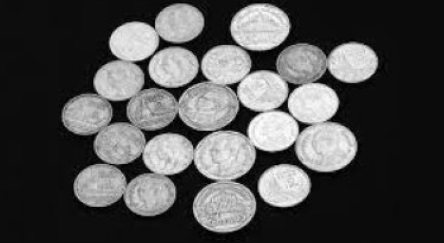
\includegraphics[width=1\textwidth]{images/input_binary_thresholding.jpg}
        \caption{Imagine de Input \cite{opencv_threshold}}
    \end{minipage}
    \hspace{0.01\textwidth}
    \begin{minipage}{0.45\textwidth}
        \centering
        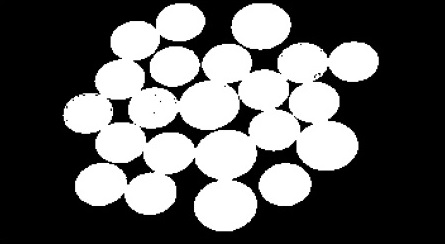
\includegraphics[width=1\textwidth]{images/output_binary_thresholding.jpg}
        \caption{Filtrul Otsu \cite{otsu1979}}
    \end{minipage}
\end{figure}
\FloatBarrier

De asemenea, este posibil ca algoritmul de binarizare să determine valoarea optimă a pragului. Aceasta se poate realiza prin utilizarea unui algoritm precum Otsu. Pe scurt, algoritmul lui Otsu ia în considerare toate pragurile posibile și calculează varianța pentru fiecare dintre cele două clase de pixeli (adică clasa de sub prag și clasa de peste prag). Algoritmul lui Otsu minimizează următoarea expresie:
\[
    \sigma_w^2 \equiv w_1(t) \cdot \sigma_1^2 + w_2(t) \cdot \sigma_2^2
\]

unde \( w_1(t) \) și \( w_2(t) \) sunt ponderile relative pentru cele două clase date de numărul de pixeli din fiecare clasă, iar \( \sigma_1^2 \) și \( \sigma_2^2 \) sunt varianțele din fiecare clasă. Se dovedește că minimizarea varianței celor două clase în acest mod este echivalentă cu maximizarea varianței între cele două clase. Deoarece este necesară o căutare exhaustivă a spațiului posibil de praguri, acest proces nu este unul foarte rapid, dar este foarte eficient în determinarea pragului optim pentru separarea pixelilor în două clase distincte.

Filtrul de binarizare prin metoda triunghi este o alta metodă eficientă pentru determinarea automată a pragului optim de binarizare a unei imagini. Această tehnică se bazează pe analiza histogramei imaginii și utilizarea unui algoritm geometric pentru a stabili punctul de prag. Procedura implică mai multe etape:

Prima etapă constă în calcularea histogramei imaginii. Fiecare intensitate este contorizată pentru a obține frecvența de apariție a fiecărei valori de pixel. După obținerea histogramei, se calculează histograma cumulativă. Aceasta ajută la identificarea distribuției totale a intensităților pixelilor și este folosită pentru a trasa linia de referință necesară în algoritmul de binarizare.

Pentru a determina linia de referință, se identifică punctele minim și maxim din histograma cumulativă. Linia de referință este trasată între aceste două puncte și servește ca bază pentru calcularea distanțelor. Pentru fiecare valoare din histograma cumulativă, se calculează distanța față de linia de referință. Această distanță este utilizată pentru a găsi punctul de pe histogramă care se află la cea mai mare distanță față de linia de referință.

Valoarea de intensitate care are cea mai mare distanță față de linia de referință este considerată pragul optim. Acest prag este folosit pentru a binariza imaginea inițială, separând pixelii în două clase: cei cu valori sub prag și cei cu valori peste prag.

Algoritmul de binarizare prin metoda triunghi oferă o metodă robustă și automată pentru binarizarea imaginilor, fiind util în diverse aplicații de prelucrare a imaginilor, unde separarea precisă a obiectelor de fundal este esențială.

\subsection*{Filtre trece-jos}

Filtrele spațiale de netezire (denumite și de mediere) sunt utilizate pentru a reduce tranzițiile abrupte în intensitate. Deoarece zgomotul aleatoriu constă de obicei din tranziții abrupte în intensitate, o metodă evidentă a netezirii este reducerea zgomotului. Netezirea înainte de resampling-ul imaginii pentru a reduce aliasing-ul este, de asemenea, o practică comună.

\begin{figure}[htbp]
    \centering
    \begin{minipage}{0.35\textwidth}
        \centering
        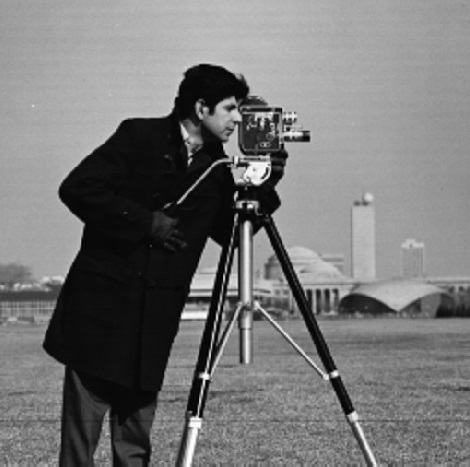
\includegraphics[width=1\textwidth]{images/input_low_pass.jpg}
        \caption{Imagine de Input \cite{opencv_gaussian}}
    \end{minipage}
    \hspace{0.01\textwidth}
    \begin{minipage}{0.35\textwidth}
        \centering
        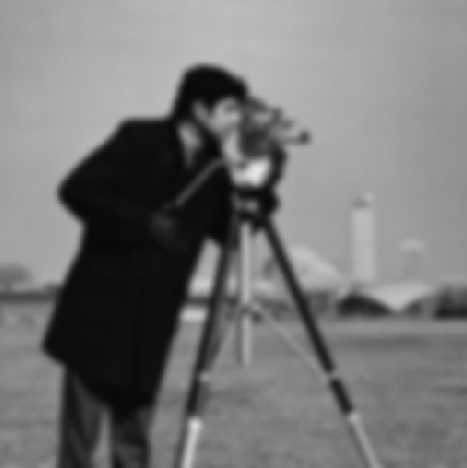
\includegraphics[width=1\textwidth]{images/output_low_pass.jpg}
        \caption{Filtrul Gaussian \cite{opencv_gaussian}}
    \end{minipage}
\end{figure}
\FloatBarrier

Netezirea este utilizată pentru a reduce detaliile nerelevante într-o imagine, unde „nerelevant” se referă la regiunile de pixeli care sunt mici în raport cu dimensiunea kernelului filtrului. O altă aplicație este netezirea contururilor false care rezultă din utilizarea unui număr insuficient de niveluri de intensitate într-o imagine. Filtrele de netezire sunt utilizate în combinație cu alte tehnici pentru îmbunătățirea imaginii, cum ar fi tehnicile de procesare a histogramelor și mascare unsharp.

Cel mai simplu filtru trece-jos separabil este filtrul de tip cutie, ale cărui coeficienți au aceeași valoare (de obicei 1). Numele „kernel cutie” provine dintr-un kernel de dimensiuni \(m \times n\) cu toți coeficienții egali. Normalizarea kernelului se face prin împărțirea fiecărui coeficient la suma valorilor coeficienților (adică \(1 / mn\) când toți coeficienții sunt 1).

Datorită simplității lor, filtrele de tip cutie sunt potrivite pentru experimentare rapidă și oferă de obicei rezultate de netezire acceptabile vizual. Cu toate acestea, filtrele de tip cutie au limitări care le fac alegeri mai puțin ideale în multe aplicații. Kernelurile Gaussian sunt utilizate frecvent datorită proprietăților lor utile și capacității de a netezi imaginile în mod eficient. Kernelurile Gaussian sunt simetrice circular (isotrope), ceea ce înseamnă că răspunsul lor este independent de orientare.

Kernelul Gaussian este dat de formula:
\[
    w(s,t) = G(s,t) = K e^{-\frac{s^2 + t^2}{2\sigma^2}}
\]

Kernelurile Gaussian sunt singurele kerneluri simetrice circular și separabile, ceea ce le conferă avantaje computaționale similare cu filtrele de tip cutie, dar cu proprietăți suplimentare care le fac ideale pentru procesarea imaginii.

Prin \(r = \sqrt{s^2 + t^2}\), putem scrie ecuația:
\[
    G(r) = K e^{-\frac{r^2}{2\sigma^2}}
\]
unde \(K\) este o constantă de normalizare, iar \(\sigma\) este deviația standard a distribuției Gaussian.

Rezultatul convoluției este deosebit de important în filtrare. De exemplu, filtrarea se poate face în etape succesive, iar același rezultat poate fi obținut printr-o singură etapă de filtrare cu un kernel compozit format ca și convoluție a kernelurilor individuale.

\subsection*{Filtre trece-sus}

Detectarea marginilor este un pas esențial, deoarece permite identificarea schimbărilor de intensitate și determinarea contururilor obiectelor. În general, detectarea marginilor implică utilizarea derivatelor de ordinul întâi sau al doilea pentru a evidenția variațiile rapide ale semnalului.

\begin{figure}[htbp]
    \centering
    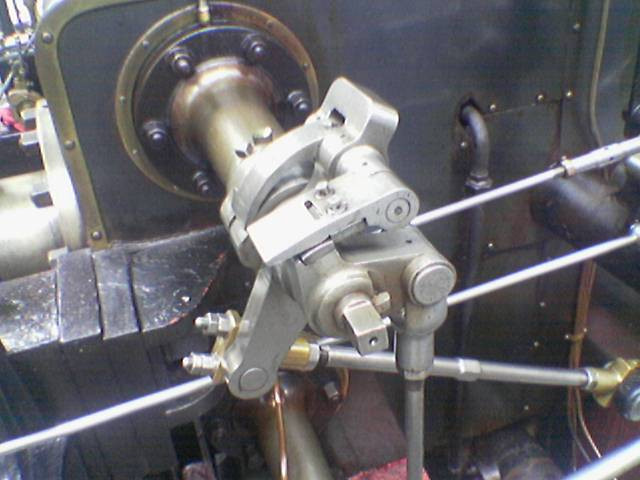
\includegraphics[width=0.4\textwidth]{images/input_edge_detection.jpg}
    \caption{Imagine de Input \cite{opencv_edges}}
\end{figure}
\FloatBarrier
\begin{figure}[htbp]
    \centering
    \begin{minipage}{0.4\textwidth}
        \centering
        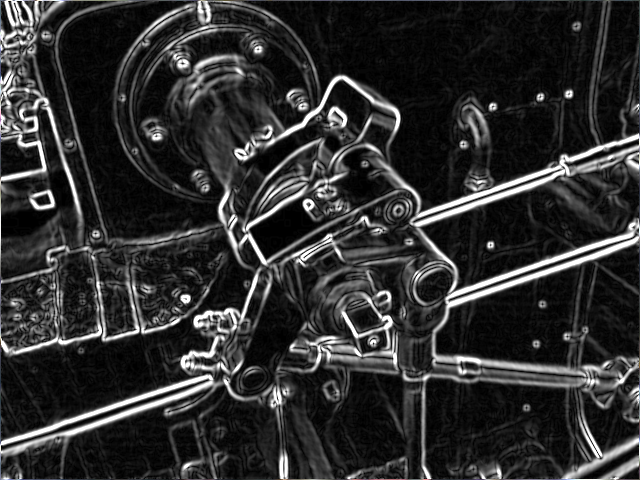
\includegraphics[width=1\textwidth]{images/sobel_edge_detection.jpg}
        \caption{Operatorul Sobel \cite{opencv_edges}}
    \end{minipage}
    \hspace{0.05\textwidth}
    \begin{minipage}{0.4\textwidth}
        \centering
        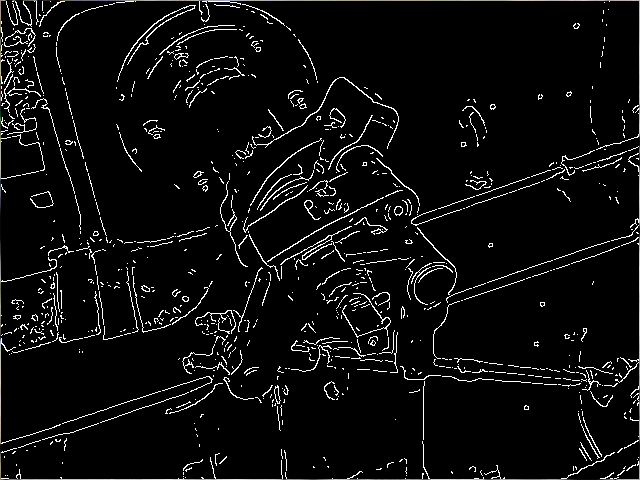
\includegraphics[width=1\textwidth]{images/canny_edge_detection.jpg}
        \caption{Filtru Laplace \cite{opencv_edges}}
    \end{minipage}
\end{figure}
\FloatBarrier

Instrumentul principal pentru determinarea direcției și intensității marginii este gradientul. Gradientul unei funcții \( f(x, y) \) este definit ca:
\[
    \nabla f(x, y) =
    \begin{bmatrix}
        g_x(x, y) \\
        g_y(x, y)
    \end{bmatrix}
\]

Magnitudinea gradientului este:
\[
    M(x, y) = \sqrt{g_x^2(x, y) + g_y^2(x, y)}
\]

Direcția gradientului este:
\[
    \alpha(x, y) = \tan^{-1}\left(\frac{g_y(x, y)}{g_x(x, y)}\right)
\]

Pentru determinarea corectă a direcției în toate cazurile, unghiul poate fi definit riguros în funcție de semnul componentelor:
\[
\alpha(x,y) =
\begin{cases}
\arctan\left(\frac{g_y}{g_x}\right) & g_x > 0 \\
\arctan\left(\frac{g_y}{g_x}\right) + \pi & g_x < 0,\, g_y \geq 0 \\
\arctan\left(\frac{g_y}{g_x}\right) - \pi & g_x < 0,\, g_y < 0 \\
\frac{\pi}{2} & g_x = 0,\, g_y > 0 \\
-\frac{\pi}{2} & g_x = 0,\, g_y < 0
\end{cases}
\]

Pentru calculul gradientului se folosesc aproximări discrete:
\[
    g_x(x, y) \approx f(x+1, y) - f(x, y)
\]
\[
    g_y(x, y) \approx f(x, y+1) - f(x, y)
\]

Operatorii Prewitt utilizează:
\[
    g_x \approx (z_7 + z_8 + z_9) - (z_1 + z_2 + z_3)
\]
\[
    g_y \approx (z_3 + z_6 + z_9) - (z_1 + z_4 + z_7)
\]

Operatorii Sobel folosesc:
\[
    g_x \approx
    \begin{bmatrix}
        -1 & 0 & 1 \\
        -2 & 0 & 2 \\
        -1 & 0 & 1
    \end{bmatrix}
\]
\[
    g_y \approx
    \begin{bmatrix}
        -1 & -2 & -1 \\
        0  & 0  & 0  \\
        1  & 2  & 1
    \end{bmatrix}
\]

Pentru a obține margini subțiri și bine definite, este necesară eliminarea valorilor care nu corespund unui maxim local. Această etapă constă în analizarea fiecărui punct în raport cu direcția gradientului.

Direcția gradientului este cuantizată, de regulă, în patru direcții principale: orizontală (0°), verticală (90°) și cele două diagonale (45° și 135°). Pentru fiecare punct, se determină direcția cea mai apropiată și se selectează doi vecini situați pe această direcție.

Valoarea punctului este comparată cu valorile acestor doi vecini:
\begin{itemize}
    \item dacă magnitudinea sa este mai mare sau egală decât ambele valori, punctul este păstrat;
    \item în caz contrar, punctul este eliminat.
\end{itemize}

Prin această operație se păstrează doar punctele care reprezintă maxime locale ale gradientului, ceea ce conduce la subțierea marginilor și eliminarea răspunsurilor multiple produse de același contur.

Gradientul morfologic este definit ca:
\[
    G = (I \oplus B) - (I \ominus B)
\]
unde \( I \) este imaginea inițială, iar \( B \) elementul structurant. Această operație evidențiază marginile prin diferența dintre dilatare și eroziune.

\subsection*{Operații morfologice}

Morfologia imaginii este un subiect de sine stătător ce cuprinde un număr mare de operații morfologice care au fost dezvoltate în special în primii ani ai viziunii computerizate. Majoritatea operațiilor au fost dezvoltate pentru un scop specific sau altul, iar unele dintre acestea și-au găsit o utilitate mai largă de-a lungul anilor. Practic, toate operațiile morfologice se bazează pe doar două operații primitive.

Transformările morfologice de bază se numesc dilatare și eroziune și apar într-o varietate de contexte, cum ar fi eliminarea zgomotului, izolarea elementelor individuale și unirea elementelor disparate într-o imagine. Operațiile morfologice mai sofisticate, bazate pe aceste două operații de bază, pot fi utilizate pentru a găsi vârfuri de intensitate (sau găuri) într-o imagine și pentru a defini (încă o dată) o formă particulară a gradientului de imagine.

\begin{figure}[htbp]
    \centering
    \begin{minipage}{0.24\textwidth}
        \centering
        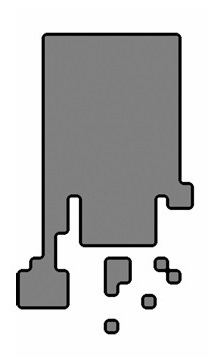
\includegraphics[width=1\textwidth]{images/input_dilate.jpg}
        \caption{Imagine de Input \cite{opencv_morphology}}
    \end{minipage}
    \hspace{0.02\textwidth}
    \begin{minipage}{0.24\textwidth}
        \centering
        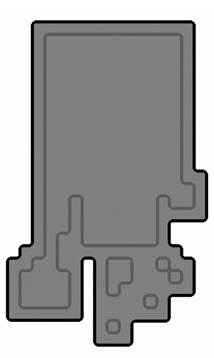
\includegraphics[width=1\textwidth]{images/output_dilate.jpg}
        \caption{Operația de dilatare \cite{opencv_morphology}}
    \end{minipage}
\end{figure}
\FloatBarrier

Dilatarea este o convoluție a unei imagini cu un nucleu în care orice pixel dat este înlocuit cu maximul local al tuturor valorilor pixelilor acoperiți de nucleu. Așa cum am menționat anterior, aceasta este un exemplu de operație neliniară, deci nucleul nu poate fi exprimat în forma arătată. Cel mai adesea, nucleul folosit pentru dilatare este un nucleu pătrat „solid” sau uneori un disc, cu punctul de ancorare în centru. Efectul dilatării este de a face ca regiunile umplute dintr-o imagine să crească.

\begin{figure}[htbp]
    \centering
    \begin{minipage}{0.24\textwidth}
        \centering
        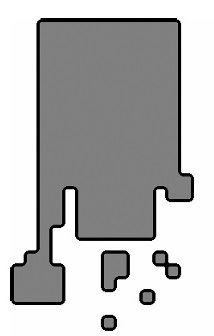
\includegraphics[width=1\textwidth]{images/input_erode.jpg}
        \caption{Imagine de Input \cite{opencv_morphology}}
    \end{minipage}
    \hspace{0.02\textwidth}
    \begin{minipage}{0.24\textwidth}
        \centering
        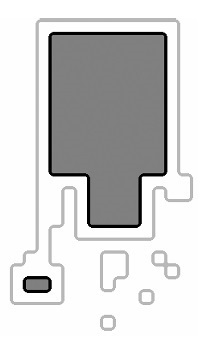
\includegraphics[width=1\textwidth]{images/output_erode.jpg}
        \caption{Operația de erodare \cite{opencv_morphology}}
    \end{minipage}
\end{figure}
\FloatBarrier

Eroziunea este operația opusă. Acțiunea operatorului de eroziune este echivalentă cu calcularea unui minim local peste zona nucleului. În general, în timp ce dilatarea extinde o regiune luminoasă, eroziunea reduce o astfel de regiune luminoasă. Mai mult, dilatarea va tinde să umple concavitățile, iar eroziunea va tinde să elimine proeminențele. Desigur, rezultatul exact va depinde de nucleu, dar aceste afirmații sunt în general adevărate atâta timp cât nucleul este convex și umplut.

\begin{figure}[htbp]
    \centering
    \begin{minipage}{0.24\textwidth}
        \centering
        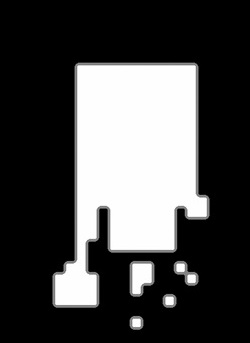
\includegraphics[width=1\textwidth]{images/input_open.jpg}
        \caption{Imagine de Input \cite{opencv_morphology}}
    \end{minipage}
    \hspace{0.02\textwidth}
    \begin{minipage}{0.24\textwidth}
        \centering
        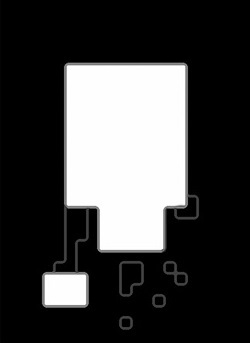
\includegraphics[width=1\textwidth]{images/output_open.jpg}
        \caption{Operația de deschidere \cite{opencv_morphology}}
    \end{minipage}
\end{figure}
\FloatBarrier

Operațiile de deschiderea și închiderea, sunt de fapt combinații simple ale operatorilor de eroziune și dilatare. În cazul deschiderii, erodăm mai întâi și apoi dilatăm. Deschiderea este adesea folosită pentru a număra regiunile într-o imagine binară. De exemplu, dacă am pragat o imagine a celulelor pe o lamă de microscop, am putea folosi deschiderea pentru a separa celulele care sunt aproape una de cealaltă înainte de a număra regiunile.

\begin{figure}[htbp]
    \centering
    \begin{minipage}{0.24\textwidth}
        \centering
        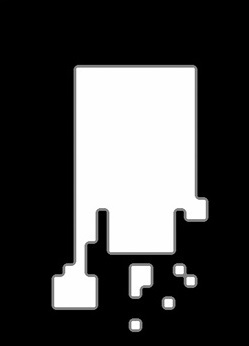
\includegraphics[width=1\textwidth]{images/input_close.jpg}
        \caption{Imagine de Input \cite{opencv_morphology}}
    \end{minipage}
    \hspace{0.02\textwidth}
    \begin{minipage}{0.24\textwidth}
        \centering
        
\includegraphics[width=1\textwidth]{images/output_close.jpg}
        \caption{Operația de închidere \cite{opencv_morphology}}
    \end{minipage}
\end{figure}
\FloatBarrier

În cazul închiderii, dilatăm mai întâi și apoi erodăm. Închiderea este utilizată în majoritatea algoritmilor de componente conexe mai sofisticați pentru a reduce segmentele nedorite sau generate de zgomot. Pentru componentele conexe, de obicei se efectuează mai întâi o eroziune sau o operație de închidere pentru a elimina elementele care apar doar din zgomot, și apoi se folosește o operație de deschidere pentru a conecta regiunile mari din apropiere. Observați că, deși rezultatul final al utilizării deschiderii sau închiderii este similar cu utilizarea eroziunii sau dilatării, aceste noi operații tind să păstreze mai precis aria regiunilor conexe.

\subsection*{Componente conexe}

Identificarea componentelor conexe este o operațiune esențială în procesarea imaginii, utilizată pentru a găsi regiuni de pixeli adiacenți care au aceeași valoare de intensitate. Aceste regiuni sunt denumite componente conexe. Pixelii sunt considerați \textit{N4}-adiacenți dacă sunt adiacenți fie orizontal, fie vertical, și \textit{N8}-adiacenți dacă pot fi și adiacenți diagonal.

Componentele conexe sunt utilizate pe scară largă în diverse aplicații, cum ar fi recunoașterea literelor dintr-un document scanat sau identificarea obiectelor (de exemplu, celule) într-o imagine segmentată și calcularea statisticilor de arie. De-a lungul anilor, au fost dezvoltate o varietate de algoritmi eficienți pentru a găsi astfel de componente. Astfel de algoritmi sunt de obicei incluși în bibliotecile de procesare a imaginii.

După ce o imagine binară sau multivalorată a fost segmentată în componentele sale conexe, este util să calculăm statisticile de arie pentru fiecare regiune individuală $\mathcal{R}$. Astfel de statistici includ:
\begin{itemize}
    \item \textbf{Aria} (numărul de pixeli);
    \item \textbf{Perimetrul} (numărul de pixeli de la margine);
    \item \textbf{Centroidul} (valorile medii $x$ și $y$);
    \item \textbf{Momentul de ordinul doi},
          \[
              M = \sum_{(x,y) \in \mathcal{R}} \begin{bmatrix}
                  x - \bar{x} \\
                  y - \bar{y}
              \end{bmatrix}
              \begin{bmatrix}
                  x - \bar{x} & y - \bar{y}
              \end{bmatrix},
          \]
          de la care se pot calcula orientarea și lungimile axelor major și minor folosind analiza valorilor proprii.
\end{itemize}

Aceste statistici pot fi apoi utilizate pentru prelucrarea ulterioară, de exemplu, pentru sortarea regiunilor în funcție de dimensiune (pentru a considera mai întâi regiunile cele mai mari) sau pentru potrivirea preliminară a regiunilor din imagini diferite.

Boxurile de delimitare sunt utilizate pentru a încadra componentele conexe identificate într-o imagine. Fiecare componentă conexă este înconjurată de un dreptunghi minim care cuprinde toți pixelii din componenta respectivă. Parametrii acestui dreptunghi sunt:
\begin{itemize}
    \item \textbf{Coordonatele colțului din stânga-sus} $(x_{min}, y_{min})$;
    \item \textbf{Lățimea și înălțimea} $(w, h)$.
\end{itemize}

Aceste boxuri de delimitare sunt esențiale în diverse aplicații de vizualizare și analiză a imaginii, oferind un mijloc simplu și eficient de localizare și izolare a componentelor de interes.

Componentelor conexe și utilizarea boxurilor de delimitare sunt instrumente fundamentale în procesarea imaginilor, permițând izolarea eficientă și analiza precisă a regiunilor de interes în imagini binare și multivalorate.

\subsection*{Analiza componentelor conexe}

După segmentarea unei imagini, de obicei prin binarizare, putem folosi analiza componentelor conexe pentru a izola și procesa eficient regiunile rezultate ale imaginii una câte una. Analiza componentelor conexe are ca scop etichetarea regiunilor conectate dintr-o imagine binară. Prin etichetarea acestor regiuni, putem izola și analiza fiecare componentă în parte.

\begin{enumerate}
    \item \textbf{Intrare}: Intrarea este o imagine binară în care prim-planul și fundalul sunt clar definite.
    \item \textbf{Etichetarea}: Fiecare pixel din prim-plan primește o etichetă, indicând care componentă conexă o reprezintă. Acest lucru are ca rezultat o hartă de pixeli etichetați unde toți pixelii din aceeași componentă conexă împărtășesc aceeași etichetă.
    \item \textbf{Ieșire}: Ieșirea este o imagine etichetată și, opțional, un set de statistici pentru fiecare componentă conexă, cum ar fi aria, dreptunghiul de delimitare și centrul de masă.
\end{enumerate}
Analiza componentelor conexe este destul de populară în algoritmii de segmentare a fundalului ca filtru post-procesare care elimină petele mici de zgomot și în probleme cum ar fi OCR, unde există un prim-plan bine definit de extras. Este esențial ca această operație de bază să fie rapidă.

\subsection*{Contururi}

Algoritmii precum detectorul de margini Canny pot fi utilizați pentru a găsi pixeli de margine care separă diferite segmente într-o imagine, dar nu ne oferă informații despre acele margini ca entități în sine. Pasul următor este să asamblăm acei pixeli de margine în contururi. Un contur este o listă de puncte care reprezintă, într-un fel sau altul, o curbă într-o imagine. Această reprezentare poate varia în funcție de circumstanțele specifice.

Există multe modalități de a reprezenta o curbă. Contururile pot fi reprezentate prin secvențe de puncte 2D. De exemplu, o astfel de reprezentare este lanțul Freeman, în care fiecare punct este reprezentat ca un „pas” într-o direcție dată de la punctul anterior. Deși secvențele de puncte 2D sunt cele mai comune, există și alte modalități de a reprezenta contururile.

Funcțiile de calcul al contururilor pornesc de la imagini binare. Acestea pot folosi imagini create de algoritmi de detectare a marginilor, cum ar fi detectorul Canny, sau imagini create prin aplicarea unor funcții de prag, în care marginile sunt implicite ca limite între regiuni pozitive și negative.

Înainte de a detalia modul de extragere a contururilor, este important să înțelegem ce este un contur și cum pot fi relaționate grupurile de contururi între ele. Un concept deosebit de important este arborele de contururi, care encodează relațiile de includere între contururi.

Un arbore de contururi este o structură ierarhică în care fiecare nod reprezintă un contur. Fiecare nod poate avea copii care sunt contururi incluse în conturul părinte. Această structură ierarhică poate fi reprezentată prin array-uri în care fiecare intrare reprezintă un contur specific. Fiecare intrare conține un set de patru întregi care indică alte noduri în ierarhie cu o relație particulară față de nodul curent. Dacă o relație specifică nu există, elementul corespunzător din structură este setat la -1 (de exemplu, ID-ul părintelui pentru nodul rădăcină ar avea valoarea -1 deoarece nu are părinte).

\begin{figure}[htbp]
    \centering
    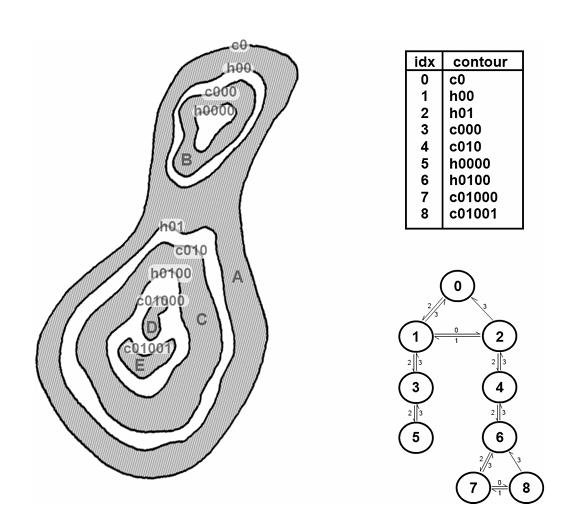
\includegraphics[width=0.75\textwidth]{images/contours.jpg}
    \caption{Regiuni \cite{opencv_contours}}
\end{figure}
\FloatBarrier

Imaginea de mai sus conține mai multe regiuni pe un fundal alb. Contururile acestor regiuni pot fi găsite și aranjate într-un arbore de contururi. De exemplu, dacă avem cinci regiuni, rezultând un total de nouă contururi (incluzând atât marginile exterioare, cât și cele interioare ale fiecărei regiuni), fiecare nod din arbore va avea ca și copii acele contururi care sunt incluse în conturul respectiv. Arborele rezultat poate fi vizualizat, arătând legăturile valide și relațiile dintre noduri.

Contururile sunt structuri esențiale în procesarea imaginii, reprezentând margini și forme într-o manieră organizată. Înțelegerea și utilizarea contururilor permite realizarea unor operațiuni avansate de analiză și manipulare a imaginii, inclusiv identificarea obiectelor și segmentarea precisă a regiunilor de interes.

\subsection*{Operații logice}

Operațiile logice lucrează cu variabile și expresii TRUE (de obicei denotate prin 1) și FALSE (de obicei denotate prin 0). În cazul nostru, aceasta înseamnă imagini binare compuse din pixeli de prim-plan (valorați cu 1) și un fundal format din pixeli cu valoarea 0.

Utilizăm operatori logici și de set pe imagini binare folosind două abordări principale:
\begin{enumerate}
    \item Utilizăm coordonatele regiunilor individuale de pixeli de prim-plan într-o singură imagine ca seturi.
    \item Lucrăm cu una sau mai multe imagini de aceeași dimensiune și efectuăm operații logice între pixelii corespunzători din aceste matrice.
\end{enumerate}

În prima categorie, o imagine binară poate fi privită ca o diagramă Venn în care coordonatele regiunilor de pixeli valorați cu 1 sunt tratate ca seturi. Uniunea acestor seturi cu setul compus din pixeli valorați cu 0 formează universul setului, Æ. De exemplu, pentru o imagine binară cu două regiuni de pixeli valorați cu 1, $R_1$ și $R_2$, putem determina dacă regiunile se suprapun (au cel puțin o pereche de coordonate comune) prin efectuarea operației de intersecție a seturilor $R_1 \cap R_2$.

În a doua abordare, efectuăm operații logice pe pixelii unei imagini binare sau pe pixelii corespunzători din două sau mai multe imagini binare de aceeași dimensiune. Operatorii logici pot fi definiți în termeni de tabele de adevăr. Operația logică AND (denotată și $\wedge$) produce 1 (TRUE) doar când ambii $a$ și $b$ sunt 1. În mod similar, OR ($\vee$) produce 1 când $a$ sau $b$ sau ambii sunt 1, iar operatorul NOT ($\neg$) este auto-explicativ. Operatorii AND și OR sunt \textit{elementwise} în acest context, operând pe perechi de pixeli corespunzători între imagini.

\begin{figure}[htbp]
    \centering
    
\includegraphics[width=0.55\textwidth]{images/logical_operations.jpg}
    \caption{Operații logice \cite{opencv_bitwise}}
\end{figure}
\FloatBarrier

Figura ilustrează operații logice folosind a doua abordare discutată. NOT al imaginii binare B1 este o matrice obținută prin schimbarea tuturor pixelilor valorați cu 1 în 0 și invers. AND dintre B1 și B2 conține 1 în toate locațiile unde elementele corespunzătoare ale B1 și B2 sunt 1; operația produce 0 în altă parte. OR dintre cele două imagini este o matrice care conține 1 în locațiile unde elementele corespunzătoare ale B1 sau B2 sau ambele sunt 1. XOR (exclusive OR) produce 1 în locațiile unde elementele corespunzătoare ale B1 sau B2 (dar nu ambele) sunt 1.

Putem obține aceleași rezultate folosind prima abordare discutată mai sus. Începem prin etichetarea regiunilor individuale valorați cu 1 în fiecare dintre cele două imagini. Să notăm cu A și B seturile de coordonate ale tuturor pixelilor valorați cu 1 în imaginile B1 și B2. Apoi formăm o singură matrice prin aplicarea operației OR între cele două imagini, păstrând etichetele A și B. Rezultatul ar arăta ca matricea $B_1 \vee B_2$, dar cu cele două regiuni albe etichetate A și B, asemănătoare unui diagramă Venn.

\subsection*{Transformări geometrice}

Utilizăm transformările geometrice pentru a modifica aranjamentul spațial al pixelilor dintr-o imagine. Transformările geometrice ale imaginilor digitale constau în două operații de bază:
\begin{enumerate}
    \item Transformarea spațială a coordonatelor.
    \item Interpolarea intensității care atribuie valori de intensitate pixelilor transformați spațial.
\end{enumerate}

Transformarea coordonatelor poate fi exprimată astfel:
\[
    \begin{bmatrix}
        x' \\
        y'
    \end{bmatrix}
    =
    T
    \begin{bmatrix}
        x \\
        y
    \end{bmatrix}
    =
    \begin{bmatrix}
        t_{11} & t_{12} \\
        t_{21} & t_{22}
    \end{bmatrix}
    \begin{bmatrix}
        x \\
        y
    \end{bmatrix}
\]
unde $(x, y)$ sunt coordonatele pixelilor în imaginea originală și $(x', y')$ sunt coordonatele pixelilor corespunzători din imaginea transformată. De exemplu, transformarea $(x', y') = (x/2, y/2)$ micșorează imaginea originală la jumătate în ambele direcții spațiale.

Ne interesează așa-numitele \textit{transformări afine}, care includ scalarea, translația, rotația și deformarea. Caracteristica principală a unei transformări afine în 2D este că păstrează punctele, liniile drepte și planele. Ecuația definită anterior poate fi folosită pentru a exprima transformările menționate mai sus, cu excepția translației, care ar necesita adăugarea unui vector constant 2D în partea dreaptă a ecuației. Cu toate acestea, este posibil să folosim coordonate omogene pentru a exprima toate cele patru transformări afine folosind o singură matrice 3x3 în următoarea formă generală:
\[
    \begin{bmatrix}
        x' \\
        y' \\
        1
    \end{bmatrix}
    =
    \begin{bmatrix}
        a_{11} & a_{12} & a_{13} \\
        a_{21} & a_{22} & a_{23} \\
        0      & 0      & 1
    \end{bmatrix}
    \begin{bmatrix}
        x \\
        y \\
        1
    \end{bmatrix}
\]

Această transformare poate scala, roti, translata sau deforma o imagine, în funcție de valorile alese pentru elementele matricei A.

Transformarea anterioară mută coordonatele pixelilor dintr-o imagine în locații noi. Pentru a finaliza procesul, trebuie să atribuim valori de intensitate pixelilor relocați. Această sarcină este realizată folosind \textit{interpolarea intensității}.

Putem utiliza ecuația în două moduri de bază. Primul este \textit{maparea directă}, care constă în scanarea pixelilor imaginii de intrare și, la fiecare locație $(x, y)$, calcularea locației spațiale $(x', y')$ a pixelului corespunzător în imaginea de ieșire folosind direct ecuația.

Al doilea mod, numit \textit{mapare inversă}, scanează locațiile pixelilor de ieșire și, la fiecare locație $(x', y')$, calculează locația corespunzătoare în imaginea de intrare folosind $(x, y) = A^{-1}(x', y')$. Apoi interpolează printre cei mai apropiați pixeli de intrare pentru a determina intensitatea valorii pixelului de ieșire.

\subsection*{Transformata Hough}

Adesea, trebuie să lucrăm în medii neorganizate în care avem doar o hartă de margini și nicio informație despre unde ar putea fi obiectele de interes. În astfel de situații, toți pixelii sunt candidați pentru legături și, astfel, trebuie să fie acceptați sau eliminați pe baza unor proprietăți globale definite. În această secțiune, dezvoltăm o abordare bazată pe faptul dacă seturile de pixeli se află pe curbe de o anumită formă. Odată detectate, aceste curbe formează marginile sau contururile regiunilor de interes.

Dat fiind $n$ puncte într-o imagine, presupunem că dorim să găsim submulțimi ale acestor puncte care se află pe linii drepte. O soluție posibilă este să găsim toate liniile determinate de fiecare pereche de puncte, apoi să găsim toate submulțimile de puncte care sunt aproape de liniile particulare. Această abordare implică găsirea $\frac{n(n-1)}{2} \sim n^2$ linii, apoi efectuarea $n \left(\frac{n(n-1)}{2}\right) \sim n^3$ comparații ale fiecărui punct pentru toate liniile.

Transformata Hough, propusă de Hough în 1962, este o metodă alternativă pentru detectarea liniilor. Fie $(x_i, y_i)$ un punct în planul $xy$ și considerăm ecuația generală a unei linii în formă de panta-interceptare: $y_i = ax_i + b$. Infinit de multe linii trec prin $(x_i, y_i)$, dar toate satisfac ecuația $y_i = ax_i + b$ pentru valori variate ale lui $a$ și $b$. Totuși, scriind această ecuație ca $b = -x_i a + y_i$ și considerând planul $ab$ (numit și spațiul parametrilor), obținem ecuația unei singure linii pentru un punct fix $(x_i, y_i)$.
\[
    x \cos \theta + y \sin \theta = \rho
\]

\begin{figure}[htbp]
    \centering
    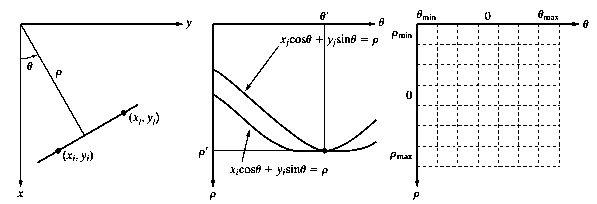
\includegraphics[width=1\textwidth]{images/hough_space.jpg}
    \caption{Interpretare geometrică \cite{opencv_hough}}
\end{figure}
\FloatBarrier

Figura ilustrează interpretarea geometrică a parametrilor $\rho$ și $\theta$. O linie orizontală are $\theta = 0^\circ$, cu $\rho$ egal cu interceptul pozitiv pe axa $x$. Similar, o linie verticală are $\theta = 90^\circ$, cu $\rho$ egal cu interceptul pozitiv pe axa $y$, sau $\theta = -90^\circ$, cu $\rho$ egal cu interceptul negativ pe axa $y$.

Atracția computațională a transformatei Hough provine din subdivizarea spațiului parametrilor $\rho, \theta$ în celule de acumulare. Procedura constă în incrementarea $\theta$ și calcularea valorilor corespunzătoare $\rho$ folosind ecuația:
\[
    \rho = x_i \cos \theta + y_i \sin \theta
\]

Celula la coordonatele $(i, j)$ cu valoare de acumulare $A(i, j)$ corespunde pătratului asociat cu coordonatele spațiului parametrilor $(\rho, \theta)$. Inițial, aceste celule sunt setate la zero. Apoi, pentru fiecare punct non-fundal $(x_k, y_k)$ în planul $xy$, incrementăm $\theta$ și calculăm $\rho$ folosind ecuația de mai sus. Valorile rezultate $\rho$ sunt rotunjite la cea mai apropiată valoare permisă de-a lungul axei $\rho$ și se actualizează celula de acumulare $A(p, q)$.

Transformata Hough este un instrument puternic pentru detectarea formelor într-o imagine și este folosită în multe aplicații practice, de la analiza imaginilor medicale la navigația autonomă.

\begin{figure}[htbp]
    \centering
    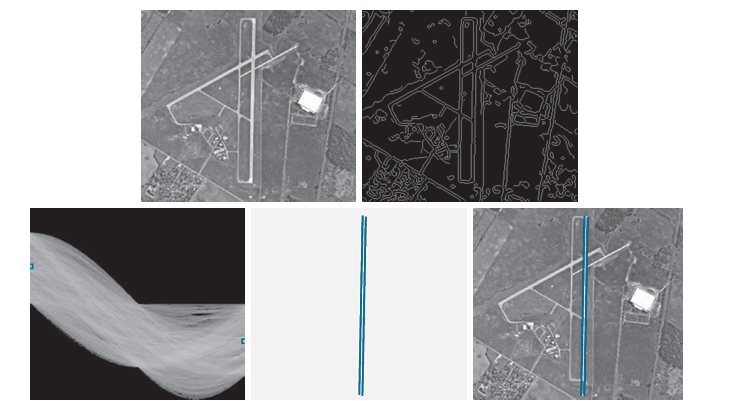
\includegraphics[width=1\textwidth]{images/airport.jpg}
    \caption{Detectarea liniilor unei piste de aterizare \cite{szeliski2010}}
\end{figure}
\FloatBarrier

Figura de mai sus arată o imagine aeriană a unui aeroport. Obiectivul acestui exemplu este să utilizăm transformata Hough pentru a extrage cele două margini care definesc pista principală. O soluție la o astfel de problemă ar putea fi de interes, de exemplu, în aplicații care implică navigația aeriană autonomă.

Primul pas este obținerea unei hărți de margini. Figura a doua arată harta de margini obținută folosind algoritmul Canny. În scopul calculării transformatei Hough, rezultate similare pot fi obținute utilizând oricare dintre celelalte tehnici de detecție a marginilor existente. Figura a treia arată spațiul parametrilor Hough obținut folosind incrementări de 1° pentru $\theta$ și incrementări de un pixel pentru $\rho$.

Pista de interes este orientată aproximativ \(1^\circ\) față de direcția nord, astfel încât selectăm celulele corespunzătoare la \(\pm 90^\circ\) și care conțin numărul cel mai mare, deoarece pistele sunt cele mai lungi linii orientate în aceste direcții. Cutiile mici de pe marginile imaginii trei evidențiază aceste celule. După cum s-a menționat anterior în legătură cu figura a doua, transformata Hough arată adiacență la marginile imaginii. O altă modalitate de interpretare a acestei proprietăți este că o linie orientată la \(+90^\circ\) și o linie orientată la \(-90^\circ\) sunt echivalente (adică, ambele sunt verticale). Imaginea a patra arată liniile corespunzătoare celor două celule de acumulare discutate anterior, iar figura a cincea arată liniile suprapuse pe imaginea originală. Liniile au fost obținute prin unirea tuturor spațiilor care nu depășesc \(20\%\) (aproximativ 100 pixeli) din înălțimea imaginii. Aceste linii corespund clar marginilor pistei de interes.

Observați că singura informație necesară pentru a rezolva această problemă a fost orientarea pistei și poziția observatorului în raport cu aceasta. Cu alte cuvinte, un vehicul care navighează autonom ar ști că, dacă pista de interes este orientată spre nord, iar direcția de deplasare a vehiculului este, de asemenea, spre nord, pista ar trebui să apară vertical în imagine. Alte orientări relative sunt tratate într-un mod similar. Orientările pistelor din întreaga lume sunt disponibile în hărțile de zbor, iar direcția de deplasare poate fi obținută cu ușurință folosind informațiile de la GPS (Global Positioning System). Aceste informații ar putea fi folosite, de asemenea, pentru a calcula distanța dintre vehicul și pistă, permițând astfel estimarea unor parametri, cum ar fi lungimea așteptată a liniilor în raport cu dimensiunea imaginii.

\subsection*{Coduri QR}

Un cod QR (\textit{Quick Response}) este o reprezentare bidimensională a informației sub forma unei matrici pătratice alcătuite din module binare. Fiecare modul poate fi interpretat ca o valoare logică:
\[
    q_{ij} \in \{0,1\}
\]
unde \(q_{ij}\) reprezintă modulul aflat pe linia \(i\) și coloana \(j\). În mod uzual, valoarea 0 corespunde unui modul alb, iar valoarea 1 unui modul negru.

Astfel, un cod QR poate fi privit ca o matrice binară:
\[
    Q =
    \begin{bmatrix}
        q_{11} & q_{12} & \cdots & q_{1N} \\
        q_{21} & q_{22} & \cdots & q_{2N} \\
        \vdots & \vdots & \ddots & \vdots \\
        q_{N1} & q_{N2} & \cdots & q_{NN}
    \end{bmatrix}
\]
unde \(N\) reprezintă numărul de module de pe o latură.

\begin{figure}[htbp]
    \centering
    
\includegraphics[width=0.25\textwidth]{images/qrcode.png}
    \caption{Exemplu de cod QR}
\end{figure}
\FloatBarrier

Dimensiunea unui cod QR depinde de versiunea acestuia. Pentru versiunea \(v\), numărul de module de pe fiecare latură este:
\[
    N = 21 + 4(v - 1)
\]
unde \(v \in \{1,2,\ldots,40\}\). Astfel, versiunea 1 are dimensiunea \(21 \times 21\), iar fiecare versiune următoare adaugă câte 4 module pe fiecare latură.

Structura unui cod QR conține atât regiuni destinate datelor, cât și regiuni auxiliare necesare localizării și decodării. Cele mai importante elemente structurale sunt marcajele de poziționare, marcajele de aliniere, zonele de sincronizare, informațiile de format, informațiile de versiune și regiunea de date.

Marcajele de poziționare sunt plasate în trei colțuri ale codului și permit determinarea poziției, orientării și scării. Acestea au o structură geometrică distinctă, formată din pătrate concentrice, ceea ce le face ușor de identificat. Marcajele de aliniere sunt utilizate pentru corectarea deformărilor geometrice, în special în cazul codurilor de dimensiuni mai mari. Zonele de sincronizare sunt secvențe alternante de module albe și negre, folosite pentru determinarea pasului grilei.

Datele sunt codificate sub forma unei secvențe binare care este plasată în matrice conform unei reguli standardizate. Înainte de plasare, secvența este completată cu biți de control pentru corecția erorilor. Dacă notăm prin \(D\) secvența de date și prin \(E\) secvența de corecție, informația totală introdusă în cod poate fi privită abstract ca:
\[
    C = D \cup E
\]
unde \(E\) introduce redundanță controlată pentru a permite recuperarea informației în cazul unor erori de citire.

Procesul de decodare presupune estimarea matricei binare \(Q\) pornind de la o imagine observată. În primul pas, se localizează marcajele de poziționare și se determină transformarea geometrică necesară pentru aducerea codului într-o formă pătratică normalizată. Apoi, regiunea rectificată este eșantionată pe o grilă de dimensiune \(N \times N\), iar fiecărui modul i se atribuie o valoare binară:
\[
    q_{ij} =
    \begin{cases}
        1, & I(i,j) < T \\
        0, & I(i,j) \geq T
    \end{cases}
\]
unde \(I(i,j)\) reprezintă intensitatea estimată a modulului, iar \(T\) este un prag de decizie.

După obținerea matricii binare, sunt extrase informațiile de format și de versiune, apoi sunt citite modulele care conțin datele propriu-zise. Dacă există erori produse de zgomot, blur, iluminare neuniformă sau deformări, acestea pot fi corectate în limita redundanței introduse prin mecanismul de corecție a erorilor.

În mod formal, decodarea poate fi privită ca o funcție:
\[
    \mathcal{D}: Q \rightarrow S
\]
unde \(Q\) este matricea binară estimată, iar \(S\) este secvența de simboluri obținută după interpretarea datelor codificate.

Robustețea unui cod QR depinde de dimensiunea modulelor, contrastul dintre clasele binare, nivelul de corecție a erorilor și precizia cu care este estimată grila. Un cod cu module bine separate, contrast ridicat și deformări geometrice reduse este mai ușor de decodat. În schimb, pierderea contrastului, zgomotul, rotația, perspectiva sau acoperirea parțială pot conduce la erori în estimarea valorilor \(q_{ij}\).

\section{Algoritmi și fundamente matematice}

\subsection*{Distanța de la un punct la o dreaptă}

Considerăm o dreaptă în planul $xy$ definită de două puncte $(x_1, y_1)$ și $(x_2, y_2)$. Ecuația generală a acestei drepte poate fi scrisă în forma:
\[
    ax + by + c = 0
\]
unde:
\begin{itemize}
    \item coeficientul $a$ este diferența dintre ordonatele celor două puncte ale dreptei:
          \[
              a = y_1 - y_2
          \]
    \item coeficientul $b$ este diferența dintre abscisele celor două puncte ale dreptei:
          \[
              b = x_2 - x_1
          \]
    \item termenul liber $c$ este dat de formula:
          \[
              c = x_1 y_2 - x_2 y_1
          \]
\end{itemize}

De asemenea, considerăm un punct $(x_0, y_0)$ în planul $xy$. Distanța de la acest punct la dreaptă este dată de formula:
\[
    d = \frac{|a x_0 + b y_0 + c|}{\sqrt{a^2 + b^2}}
\]

Această formulă ne permite să calculăm distanța perpendiculară de la un punct dat la o dreaptă specificată prin două puncte în planul $xy$.

\subsection*{Punctul de intersecție a două drepte}


Considerăm două drepte în planul $xy$, fiecare definită de două puncte. Prima dreaptă este definită de punctele $(x_1, y_1)$ și $(x_2, y_2)$, iar a doua dreaptă este definită de punctele $(x_3, y_3)$ și $(x_4, y_4)$.

Ecuația generală a unei drepte în planul $xy$ poate fi scrisă în forma:
\[
    Ax + By = C
\]

Pentru prima dreaptă, ecuația este:
\[
    A_1 x + B_1 y = C_1
\]
unde:
\[
    A_1 = y_2 - y_1, \quad B_1 = x_1 - x_2, \quad C_1 = A_1 x_1 + B_1 y_1
\]

Pentru a doua dreaptă, ecuația este:
\[
    A_2 x + B_2 y = C_2
\]
unde:
\[
    A_2 = y_4 - y_3, \quad B_2 = x_3 - x_4, \quad C_2 = A_2 x_3 + B_2 y_3
\]

Punctul de intersecție $(x, y)$ al celor două drepte poate fi determinat rezolvând sistemul de ecuații liniare:
\[
    \begin{cases}
        A_1 x + B_1 y = C_1 \\
        A_2 x + B_2 y = C_2
    \end{cases}
\]

Pentru a rezolva acest sistem, folosim determinantul:
\[
    D = A_1 B_2 - A_2 B_1
\]

Dacă $D \neq 0$, sistemul are o soluție unică, iar coordonatele punctului de intersecție sunt date de:
\[
    x = \frac{B_2 C_1 - B_1 C_2}{D}
\]
\[
    y = \frac{A_1 C_2 - A_2 C_1}{D}
\]

Dacă $D = 0$, dreptele sunt paralele și nu se intersectează într-un punct finit.

\subsection*{Distanța euclidiană}

Distanța euclidiană măsoară separarea geometrică directă dintre două puncte. Aceasta este utilă atunci când dorim să cuantificăm cât de „departe” se află două puncte caracteristice, două centre de obiecte sau două regiuni dintr-o imagine.

Considerăm două puncte dintr-o imagine:
\[
    P_1 = (x_1, y_1), \quad P_2 = (x_2, y_2)
\]

Distanța euclidiană dintre ele este:
\[
    d_E(P_1, P_2) =
    \sqrt{(x_2 - x_1)^2 + (y_2 - y_1)^2}
\]

Această valoare reprezintă lungimea segmentului care unește cele două puncte. Spre deosebire de măsurile bazate pe deplasări orizontale și verticale separate, distanța euclidiană ia în considerare simultan variația pe ambele axe.

\subsection*{Distanța dintre două drepte}

Considerăm două drepte în planul $xy$. Prima dreaptă este definită de coordonatele $(x_1, y_1)$ și $(x_2, y_2)$, iar a doua dreaptă de referință este definită de coordonatele $(x_r, y_r)$ și $(x_s, y_s)$.

Pentru a determina poziția relativă a unei drepte față de dreapta de referință, mai întâi calculăm punctul mediu al primei drepte. Coordonatele punctului mediu $(x_m, y_m)$ sunt date de:

\[
    x_m = \frac{x_1 + x_2}{2}
\]
\[
    y_m = \frac{y_1 + y_2}{2}
\]

Distanța dintre punctul mediu $(x_m, y_m)$ și dreapta de referință este calculată folosind formula:
\[
    d = (x_m - x_r) \cdot (y_s - y_r) - (y_m - y_r) \cdot (x_s - x_r)
\]

Această formulă este derivată din proprietățile determinantului și reprezintă o măsură a distanței semnate dintre punctul mediu și dreapta de referință. Semnul distanței indică poziția relativă a punctului mediu față de dreapta de referință. Astfel:
\begin{itemize}
    \item dacă $d > 0$, punctul mediu $(x_m, y_m)$ se află de o parte a dreptei de referință,
    \item  dacă $d < 0$, punctul mediu $(x_m, y_m)$ se află de cealaltă parte a dreptei de referință,
    \item  dacă $d = 0$, punctul mediu $(x_m, y_m)$ se află exact pe dreapta de referință.
\end{itemize}

\subsection*{Determinarea unei drepte care trece printr-un punct}

Considerăm un punct dat $(x_0, y_0)$ în planul $xy$ și o pantă $m$. Obiectivul este de a determina ecuația dreptei care trece prin acest punct și are panta specificată.

Ecuația generală a unei drepte în planul $xy$ este dată de:
\[
    y = mx + b
\]
unde $m$ este panta dreptei și $b$ este interceptul pe axa $y$.

Pentru a determina interceptul $b$, utilizăm coordonatele punctului $(x_0, y_0)$. Substituim aceste coordonate în ecuația generală a dreptei:
\[
    y_0 = mx_0 + b
\]

Rezolvăm pentru $b$:
\[
    b = y_0 - mx_0
\]

Pentru a determina punctele de start și de sfârșit ale dreptei în cadrul unui sistem de coordonate de dimensiune $(W, H)$, procedăm în funcție de direcția în care dorim să extindem dreapta.
\begin{enumerate}
    \item Extinderea dreptei pe direcția orizontală
          \begin{itemize}
              \item Punctul de start $(x_s, y_s)$:
                    \[
                        x_s = 0, \quad y_s = b
                    \]
              \item Punctul de sfârșit $(x_e, y_e)$:
                    \[
                        x_e = W, \quad y_e = mW + b
                    \]
          \end{itemize}
    \item Extinderea dreptei pe direcția verticală
          \begin{itemize}
              \item  Dacă $m \neq 0$:
                    \begin{itemize}

                        \item Punctul de start $(x_s, y_s)$:
                              \[
                                  x_s = -\frac{b}{m}, \quad y_s = 0
                              \]
                        \item Punctul de sfârșit $(x_e, y_e)$:
                              \[
                                  x_e = \frac{H - b}{m}, \quad y_e = H
                              \]
                    \end{itemize}
              \item Dacă $m = 0$:
                    \begin{itemize}
                        \item Punctul de start $(x_s, y_s)$ și punctul de sfârșit $(x_e, y_e)$:
                              \[
                                  x_s = x_e = x_0, \quad y_s = 0, \quad y_e = H
                              \]
                    \end{itemize}

          \end{itemize}
\end{enumerate}

Astfel, ecuația dreptei și punctele de start și sfârșit pot fi determinate folosind panta $m$ și punctul dat $(x_0, y_0)$. Acest proces ne permite să trasăm o dreaptă definită clar în cadrul unui sistem de coordonate specificat.

\subsection*{Logica fuzzy}

Logica fuzzy reprezintă o extindere a logicii clasice (booleene), în care valorile de adevăr nu sunt limitate la cele două stări discrete \(0\) (fals) și \(1\) (adevărat), ci pot lua valori continue într-un interval:
\[
    \mu(x) \in [0, 1]
\]

În acest context, un element poate aparține unui set într-o anumită măsură, descrisă printr-o funcție de apartenență \( \mu \). Astfel, în loc de a afirma că un element aparține sau nu unei mulțimi, logica fuzzy permite exprimarea gradului de apartenență.

De exemplu, în loc să considerăm că o temperatură este „ridicată” sau „nu este ridicată”, putem spune că aceasta este „ridicată” într-o proporție de \(0.7\), reflectând natura graduală a conceptului.

Un set fuzzy \(A\) este definit ca:
\[
    A = \{(x, \mu_A(x)) \mid x \in X\}
\]
unde \(X\) este universul de discurs, iar \(\mu_A(x)\) este funcția de apartenență.

Operațiile logice clasice sunt generalizate în logica fuzzy:
\begin{itemize}
    \item \textbf{AND (intersecție)}:
    \[
        \mu_{A \cap B}(x) = \min(\mu_A(x), \mu_B(x))
    \]
    \item \textbf{OR (reuniune)}:
    \[
        \mu_{A \cup B}(x) = \max(\mu_A(x), \mu_B(x))
    \]
    \item \textbf{NOT (complement)}:
    \[
        \mu_{\neg A}(x) = 1 - \mu_A(x)
    \]
\end{itemize}

Logica fuzzy este utilizată pentru modelarea incertitudinii și a conceptelor vagi, fiind aplicabilă în sisteme de control, procesarea semnalelor și luarea deciziilor, unde limitele rigide ale logicii clasice nu sunt adecvate.

\section{Învățare automată}

\subsection*{Paradigme ale învățării automate}

Învățarea automată poate fi clasificată în mai multe paradigme, în funcție de tipul datelor disponibile și de modul în care este definit semnalul de învățare. În mod general, se consideră un model parametrizat \( f_\theta \), unde \( \theta \) reprezintă parametrii ajustați pe baza datelor.

Principalele paradigme ale învățării automate sunt:

\begin{itemize}
    \item \textbf{Învățarea supervizată} utilizează un set de date etichetat:
    \[
        \mathcal{D} = \{(x_i, y_i)\}_{i=1}^{N}
    \]
    unde \( x_i \) reprezintă datele de intrare, iar \( y_i \) reprezintă etichetele asociate. Scopul este învățarea unei funcții:
    \[
        f_\theta : \mathcal{X} \rightarrow \mathcal{Y}
    \]
    care să modeleze relația dintre intrări și ieșiri. Această paradigmă este utilizată în probleme precum clasificarea și regresia.

    \item \textbf{Învățarea nesupervizată} operează pe date fără etichete:
    \[
        \mathcal{D} = \{x_i\}_{i=1}^{N}
    \]
    și urmărește descoperirea unor structuri interne ale datelor, cum ar fi grupuri, regularități sau reprezentări compacte. Un exemplu este definirea unei reprezentări latente:
    \[
        z_i = g_\phi(x_i)
    \]
    unde \( z_i \) surprinde caracteristici esențiale ale datelor.

    \item \textbf{Învățarea semi-supervizată} combină un set redus de date etichetate cu un set mai mare de date neetichetate:
    \[
        \mathcal{D} = \mathcal{D}_L \cup \mathcal{D}_U
    \]
    unde:
    \[
        \mathcal{D}_L = \{(x_i, y_i)\}, \quad
        \mathcal{D}_U = \{x_j\}
    \]
    Această paradigmă exploatează informația structurală din datele neetichetate pentru a îmbunătăți modelarea relației dintre intrări și ieșiri.

    \item \textbf{Învățarea auto-supervizată} reprezintă o abordare în care etichetele sunt generate automat din date. Se pornește de la un set neetichetat:
    \[
        \mathcal{D} = \{x_i\}_{i=1}^{N}
    \]
    și se construiesc sarcini auxiliare în care o parte din date este utilizată pentru a prezice o altă parte sau o transformare a acesteia. Scopul este obținerea unor reprezentări relevante ale datelor.

    \item \textbf{Învățarea prin recompensă} implică un agent care interacționează cu un mediu. La fiecare pas, agentul se află într-o stare \( s_t \), alege o acțiune \( a_t \) și primește un semnal de recompensă \( r_t \). Evoluția sistemului poate fi descrisă printr-o secvență:
    \[
        (s_0, a_0, r_0, s_1, a_1, r_1, \ldots)
    \]
    Scopul este determinarea unei strategii de acțiune:
    \[
        \pi(a|s)
    \]
    care conduce la un comportament optim în timp, ținând cont de efectele cumulative ale acțiunilor.
\end{itemize}

\subsection*{Tipuri de probleme în învățarea automată}

În cadrul învățării automate, problemele pot fi clasificate în funcție de natura ieșirii dorite și de obiectivul urmărit. În mod general, se consideră un set de date de intrare \( \mathcal{D} \), iar scopul este modelarea unei relații sau extragerea unor proprietăți relevante ale datelor.

Principalele tipuri de probleme sunt:

\begin{itemize}
    \item \textbf{Clasificarea} presupune atribuirea fiecărui exemplu de intrare unei clase dintr-un set finit de categorii:
    \[
        y \in \{1, 2, \ldots, C\}
    \]
    unde \( C \) este numărul total de clase. Modelul învață o funcție:
    \[
        f_\theta : \mathcal{X} \rightarrow \{1, \ldots, C\}
    \]
    care asociază fiecărei intrări \( x \) o etichetă discretă. Clasificarea poate fi binară (\(C=2\)) sau multiclasă (\(C > 2\)).

    \item \textbf{Regresia} implică estimarea unei valori numerice continue:
    \[
        y \in \mathbb{R}
    \]
    sau, mai general,
    \[
        y \in \mathbb{R}^k
    \]
    pentru cazul multivariabil. Modelul aproximează o funcție:
    \[
        f_\theta : \mathcal{X} \rightarrow \mathbb{R}
    \]
    care descrie dependența dintre variabilele de intrare și o mărime continuă.

    \item \textbf{Clusteringul} este o problemă nesupervizată care constă în gruparea datelor în submulțimi (clustere) astfel încât elementele din același grup să fie similare între ele, iar elementele din grupuri diferite să fie cât mai distincte. Formal, se caută o partiționare:
    \[
        \mathcal{D} = \bigcup_{k=1}^{K} \mathcal{C}_k
    \]
    unde \( \mathcal{C}_k \) sunt clusterele, iar:
    \[
        \mathcal{C}_i \cap \mathcal{C}_j = \emptyset \quad \text{pentru } i \neq j
    \]
    Similaritatea este de obicei definită printr-o măsură de distanță, cum ar fi distanța euclidiană.

    \item \textbf{Reducerea dimensionalității} urmărește transformarea datelor dintr-un spațiu de dimensiune mare într-un spațiu de dimensiune mai mică, păstrând cât mai mult din informația relevantă. Fie:
    \[
        x \in \mathbb{R}^d
    \]
    o intrare inițială. Se caută o transformare:
    \[
        z = g(x), \quad z \in \mathbb{R}^m, \quad m < d
    \]
    unde \( z \) este o reprezentare de dimensiune redusă. Această transformare poate fi utilizată pentru vizualizare, compresie sau eliminarea redundanței din date.
\end{itemize}

\subsection*{Rețele neuronale}

Rețelele neuronale artificiale reprezintă o clasă de modele de învățare automată inspirate din structura sistemului nervos biologic. Acestea sunt alcătuite din unități de calcul simple, interconectate, care procesează informația prin transformări succesive. Scopul unei rețele neuronale este de a aproxima o funcție:
\[
    f_\theta : \mathcal{X} \rightarrow \mathcal{Y}
\]
unde \( \theta \) reprezintă parametrii modelului, învățați din date.

\begin{figure}[htbp]
    \centering
    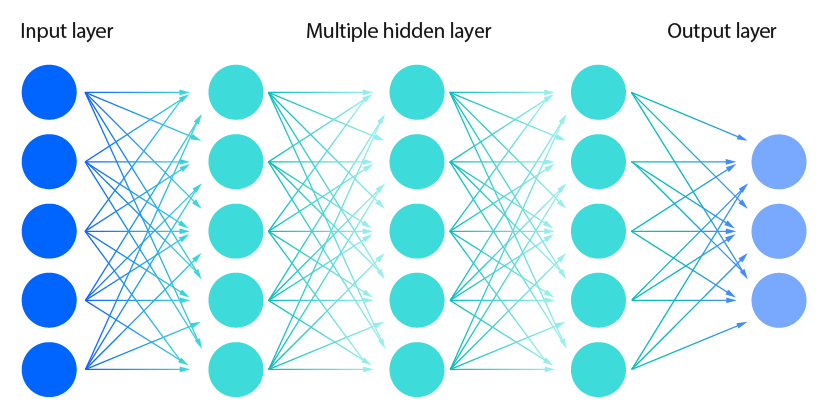
\includegraphics[width=0.8\textwidth]{images/mlp.png}
    \caption{Model de rețea neuronală \cite{nn_playground}}
\end{figure}
\FloatBarrier

Neuronul artificial este unitatea de bază a unei rețele neuronale. Acesta primește un vector de intrare:
\[
    x = (x_1, x_2, \ldots, x_n)
\]
și produce o ieșire prin aplicarea unei combinații liniare urmate de o funcție de activare:
\[
    z = \sum_{i=1}^{n} w_i x_i + b
\]
\[
    y = \sigma(z)
\]
unde \( w_i \) sunt ponderile, \( b \) este termenul de bias, iar \( \sigma \) este funcția de activare.

Perceptronul este cea mai simplă formă de neuron utilizată pentru clasificare liniară. Ieșirea sa este determinată de semnul combinației liniare:
\[
    y =
    \begin{cases}
        1, & \text{dacă } \sum_{i=1}^{n} w_i x_i + b \geq 0 \\
        0, & \text{altfel}
    \end{cases}
\]
Perceptronul poate separa doar date liniar separabile, fiind limitat în modelarea relațiilor complexe.

Straturile (layers) sunt grupuri de neuroni organizați pe niveluri. O rețea neuronală este formată, în mod tipic, din:
\begin{itemize}
    \item un strat de intrare, care primește datele;
    \item unul sau mai multe straturi ascunse, care realizează transformări intermediare;
    \item un strat de ieșire, care produce rezultatul final.
\end{itemize}

Transformarea realizată de un strat poate fi exprimată sub formă matricială:
\[
    h = \sigma(Wx + b)
\]
unde \( W \) este matricea ponderilor, \( b \) vectorul de bias, iar \( \sigma \) este aplicată element cu element.

Perceptronul multistrat (MLP) este o rețea neuronală formată din mai multe straturi complet conectate. Ieșirea fiecărui strat devine intrarea stratului următor:
\[
    h^{(l)} = \sigma\left(W^{(l)} h^{(l-1)} + b^{(l)}\right)
\]
unde \( l \) indică stratul curent, iar \( h^{(0)} = x \) este intrarea inițială.

MLP-urile sunt capabile să aproximeze funcții neliniare complexe datorită compunerii mai multor transformări și a utilizării funcțiilor de activare neliniare. Acestea stau la baza multor aplicații moderne de învățare automată.

\subsection*{Rețele neuronale convoluționale (CNN)}

Rețelele neuronale profunde (DNN) reprezintă modele compuse din mai multe straturi de procesare, capabile să învețe reprezentări ierarhice ale datelor. Aceste modele extind perceptronul multistrat prin adăugarea de profunzime și capacitate de modelare a relațiilor complexe.

Rețelele neuronale convoluționale (CNN) reprezintă o clasă particulară de DNN specializată în procesarea datelor cu structură spațială, cum ar fi imaginile. Spre deosebire de rețelele complet conectate, CNN-urile exploatează relațiile locale dintre elemente și folosesc parametri partajați pentru a reduce complexitatea modelului.

\begin{figure}[htbp]
    \centering
    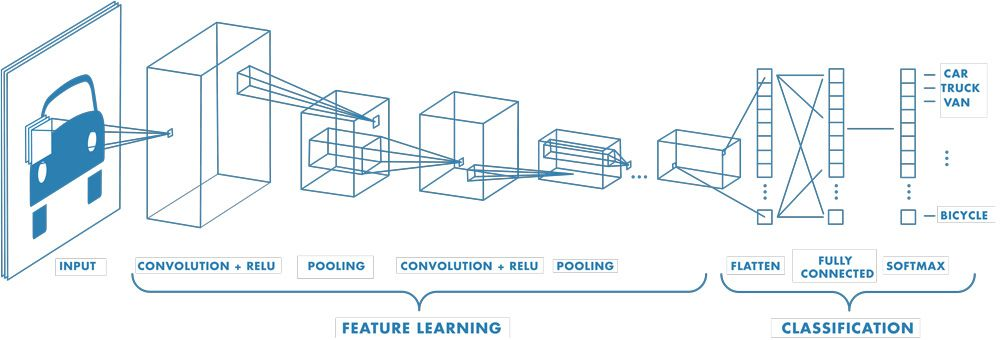
\includegraphics[width=0.8\textwidth]{images/cnn.jpg}
    \caption{Model de rețea neuronală convolutională \cite{cnn_cs231n}}
\end{figure}
\FloatBarrier

Convoluția și corelația sunt operațiile fundamentale din cadrul CNN-urilor. În practică, majoritatea implementărilor utilizează corelația, care poate fi exprimată pentru o imagine \( I \) și un nucleu \( K \) astfel:
\[
    (I * K)(x, y) =
    \sum_{i} \sum_{j}
    I(x+i, y+j) \cdot K(i, j)
\]
Această operație produce o nouă imagine în care fiecare valoare este rezultatul unei combinații locale între imaginea de intrare și nucleu. Convoluția matematică diferă prin inversarea nucleului, însă în contextul CNN-urilor diferența nu afectează în mod esențial rezultatul învățării.

Nucleul (numit și kernel, mască sau filtru) este o matrice de dimensiuni reduse:
\[
    K \in \mathbb{R}^{m \times n}
\]
care este aplicată pe întreaga imagine. Valorile kernelului sunt parametri învățați și au rolul de a detecta anumite tipare locale, cum ar fi margini, texturi sau alte caracteristici relevante. Același nucleu este utilizat pe întreaga imagine, ceea ce implică partajarea parametrilor.

Pasul reprezintă deplasarea cu care kernelul este mutat peste imagine. Dacă pasul este \( s \), atunci kernelul este mutat cu \( s \) pixeli la fiecare pas pe direcțiile orizontală și verticală. Formal, pozițiile evaluate sunt:
\[
    x = ks, \quad y = ls
\]
unde \( k, l \in \mathbb{Z} \). Un pas mai mare reduce dimensiunea rezultatului și implicit costul computațional, dar poate duce la pierderea unor detalii fine.

Hărți de caracteristici sunt rezultatele aplicării unui nucleu asupra imaginii de intrare. Fiecare nucleu produce o hartă de caracteristici:
\[
    F_k = I * K_k
\]
unde \( K_k \) este al \(k\)-lea nucleu. Aceste hărți evidențiază prezența anumitor caracteristici în diferite regiuni ale imaginii. Într-un strat convoluțional, utilizarea mai multor măști conduce la obținerea unui set de hărți de caracteristici, care sunt apoi utilizate ca intrare pentru straturile următoare.

Pentru reducerea dimensionalității și păstrarea caracteristicilor relevante, în CNN-uri se utilizează frecvent operații de tip \textit{pooling}. Una dintre cele mai comune este \textit{max pooling}, care selectează valoarea maximă dintr-o regiune locală:
\[
    P(x, y) = \max_{(i,j) \in \mathcal{N}(x,y)} I(i,j)
\]
unde \( \mathcal{N}(x,y) \) reprezintă vecinătatea locală (de exemplu, o fereastră \(2 \times 2\) sau \(3 \times 3\)). Această operație reduce dimensiunea spațială a datelor și contribuie la obținerea unor reprezentări mai robuste la variații locale.

Pe măsură ce rețelele devin mai adânci, apare problema degradării performanței. Pentru a combate acest fenomen, sunt utilizate arhitecturi cu conexiuni reziduale. Ideea de bază este învățarea unei funcții reziduale:
\[
    y = F(x) + x
\]
unde \( x \) este intrarea într-un bloc, iar \( F(x) \) reprezintă transformarea învățată. Aceste residual blocks facilitează propagarea gradientului și permit antrenarea unor rețele mult mai profunde.

Prin aplicarea succesivă a acestor operații — convoluții, pooling și conexiuni reziduale — CNN-urile construiesc reprezentări din ce în ce mai abstracte ale datelor, pornind de la caracteristici simple (cum ar fi margini) și ajungând la structuri complexe relevante pentru sarcina analizată.

\subsection*{Antrenarea unui model}

Procesul de antrenare al unui model de învățare automată constă în ajustarea parametrilor acestuia astfel încât să aproximeze cât mai bine relația dintre datele de intrare și ieșirile dorite. Acest proces este iterativ și implică mai multe etape fundamentale.

Prima etapă este propagarea înainte. În această fază, datele de intrare \( x \) sunt propagate prin rețea strat cu strat, utilizând transformări liniare și funcții de activare. Pentru un strat generic, ieșirea este:
\[
z = Wx + b, \quad a = \sigma(z)
\]
unde \( W \) și \( b \) sunt parametrii modelului, iar \( \sigma \) este funcția de activare.

Funcția de activare introduce neliniaritate în model, permițând rețelei să învețe relații complexe. Exemple comune includ funcția \textit{ReLU}:
\[
\sigma(z) = \max(0, z)
\]
și funcția sigmoidă:
\[
\sigma(z) = \frac{1}{1 + e^{-z}}
\]
care comprimă valorile în intervalul \([0,1]\), fiind frecvent utilizată în probleme de clasificare binară.

O alternativă modernă este funcția \textit{SiLU}, definită ca:
\[
\sigma(z) = z \cdot \frac{1}{1 + e^{-z}}
\]
Aceasta combină comportamentul liniar cu proprietățile funcției sigmoide, conducând în practică la o convergență mai stabilă și performanțe îmbunătățite în rețele profunde.

În cadrul propagării înainte, este frecvent utilizată și normalizarea activărilor pentru stabilizarea procesului de antrenare. O astfel de tehnică este normalizarea pe grupuri, care împarte canalele în grupuri și normalizează fiecare grup separat:
\[
\hat{x}_i = \frac{x_i - \mu_G}{\sqrt{\sigma_G^2 + \epsilon}}
\]
unde \( \mu_G \) și \( \sigma_G^2 \) sunt media și varianța calculate pe grupul \( G \). Această metodă este mai robustă decât normalizarea pe loturi în situații în care dimensiunea seturilor de date procesate simultan este redusă.

După propagarea înainte, se obține o predicție \( \hat{y} \). Aceasta este comparată cu valoarea reală \( y \) folosind o funcție de cost sau funcție de pierdere, care cuantifică eroarea modelului. De exemplu, pentru regresie:
\[
\mathcal{L}(y, \hat{y}) = (y - \hat{y})^2
\]
iar pentru clasificare se utilizează frecvent entropia încrucișată.

Pentru a îmbunătăți modelul, este necesar să ajustăm parametrii astfel încât valoarea funcției de pierdere să fie minimizată. Acest lucru se realizează prin propagarea înapoi, un algoritm care calculează derivata funcției de cost în raport cu fiecare parametru al modelului.

Elementul central în acest proces este gradientul, care indică direcția în care funcția de cost crește cel mai rapid. Pentru a minimiza pierderea, parametrii sunt actualizați în direcția opusă gradientului:
\[
\theta \leftarrow \theta - \eta \nabla_\theta \mathcal{L}
\]
unde \( \eta \) este rata de învățare.

Funcția de optimizare definește modul în care sunt actualizați parametrii pe baza gradientului. Cel mai simplu algoritm este coborârea pe gradient, însă există variante mai avansate precum Adam, RMSProp sau coborârea stochastică pe gradient cu moment, care accelerează convergența și îmbunătățesc stabilitatea antrenării.

Aceste etape, adică propagarea înainte, calculul pierderii, propagarea înapoi și actualizarea parametrilor, sunt repetate iterativ până când modelul atinge o performanță satisfăcătoare.

\subsection*{Tehnici de regularizare}

În procesul de învățare a unui model, pot apărea două probleme fundamentale: \textit{underfitting} și \textit{overfitting}.

Underfitting apare atunci când modelul este prea simplu pentru a captura structura datelor. În acest caz, modelul nu reușește să învețe relațiile relevante, având performanțe slabe atât pe datele de antrenare, cât și pe date noi. Formal, modelul nu aproximează adecvat funcția țintă:
\[
    f_\theta(x) \not\approx y
\]

Overfitting apare atunci când modelul este prea complex și învață nu doar structura generală a datelor, ci și zgomotul specific setului de antrenare. Astfel, modelul obține performanțe foarte bune pe datele de antrenare, dar generalizează slab pe date nevăzute.

Regularizarea reprezintă un ansamblu de tehnici utilizate pentru a controla complexitatea modelului și a preveni overfitting-ul. Ideea principală este de a impune constrângeri asupra parametrilor modelului, astfel încât acesta să învețe soluții mai simple și mai robuste.

O abordare comună este penalizarea valorilor mari ale parametrilor. De exemplu, în regularizarea de tip \(L2\), se adaugă un termen proporțional cu norma pătratică a parametrilor:
\[
    \|\theta\|_2^2 = \sum_{i} \theta_i^2
\]

Un hiperparametru important asociat acestei tehnici este decăderea ponderilor, notat de obicei cu \( \lambda \). Acesta controlează intensitatea penalizării:
\begin{itemize}
    \item valori mici ale lui \( \lambda \) duc la o regularizare slabă;
    \item valori mari ale lui \( \lambda \) forțează parametrii să fie mici, reducând complexitatea modelului.
\end{itemize}

Prin alegerea adecvată a acestui hiperparametru, se poate obține un echilibru între capacitatea de învățare a modelului și abilitatea sa de generalizare.

Pe lângă penalizarea parametrilor, există și alte tehnici de regularizare, cum ar fi reducerea dimensiunii modelului, utilizarea unor seturi de date mai mari sau introducerea de zgomot controlat în procesul de antrenare. Toate aceste metode urmăresc același obiectiv: îmbunătățirea performanței modelului pe date noi, nevăzute anterior.

\subsection*{Hiperparametri}

Hiperparametrii sunt valori configurate înainte de începerea procesului de antrenare și care nu sunt învățate direct din date. Aceștia controlează comportamentul modelului și al algoritmului de antrenare.

Spre deosebire de parametrii modelului, cum ar fi ponderile și termenii de bias, hiperparametrii trebuie aleși manual sau prin proceduri automate. Alegerea lor influențează semnificativ performanța finală a modelului.

Câțiva hiperparametri importanți sunt: numărul de epoci, care reprezintă numărul de treceri complete prin întregul set de date de antrenare (un număr prea mic poate duce la subînvățare, iar unul prea mare la supraînvățare), și rata de învățare (\( \eta \)), care controlează dimensiunea pasului cu care sunt actualizați parametrii în timpul optimizării:
\[
\theta_{t+1} = \theta_t - \eta \nabla_\theta \mathcal{L}
\]
De asemenea, există și alți hiperparametri relevanți, precum dimensiunea lotului, factorul de regularizare sau arhitectura rețelei, care influențează semnificativ procesul de antrenare și performanța modelului.

Determinarea valorilor optime pentru hiperparametri se poate realiza printr-un proces numit ajustarea hiperparametrilor. Formal, problema poate fi formulată ca:
\[
\theta^* = \arg\min_{\theta \in \Theta} \mathcal{L}_{val}(\theta)
\]
unde \( \Theta \) este spațiul hiperparametrilor, iar \( \mathcal{L}_{val} \) este eroarea pe setul de validare.

Pentru o estimare mai robustă a performanței, se utilizează frecvent validarea încrucișată. Aceasta presupune împărțirea setului de date în \( K \) subseturi aproximativ egale:
\[
\mathcal{D} = \bigcup_{k=1}^{K} \mathcal{D}_k
\]
Modelul este antrenat de \( K \) ori, de fiecare dată folosind \( K-1 \) subseturi pentru antrenare și unul pentru validare. Eroarea finală este obținută ca medie:
\[
\mathcal{L}_{cv} = \frac{1}{K} \sum_{k=1}^{K} \mathcal{L}^{(k)}
\]
unde \( \mathcal{L}^{(k)} \) reprezintă eroarea obținută la pasul \( k \). Această metodă reduce dependența de o singură împărțire a datelor și oferă o evaluare mai stabilă a performanței modelului.

Metodele simple de ajustare includ căutarea în grilă, unde se testează exhaustiv combinații:
\[
\Theta = \{\eta_1, \eta_2, \ldots\} \times \{E_1, E_2, \ldots\}
\]
și căutarea aleatorie, unde hiperparametrii sunt eșantionați:
\[
\theta \sim P(\Theta)
\]

Totuși, aceste metode pot deveni rapid ineficiente pe măsură ce spațiul de căutare crește. Din acest motiv, în practică se folosesc metode de optimizare inteligentă, precum optimizarea bayesiană. Aceasta construiește un model probabilistic al funcției obiectiv:
\[
p(\mathcal{L} \mid \theta)
\]
și alege următorii hiperparametri prin maximizarea unei funcții de achiziție:
\[
\theta_{next} = \arg\max_{\theta} a(\theta)
\]

Prin aceste metode, explorarea spațiului hiperparametrilor devine mai eficientă, fiind posibilă identificarea unor configurații aproape optime cu un număr redus de experimente.

Alegerea corectă a hiperparametrilor este esențială pentru obținerea unui model performant și robust.

\subsection*{Setul de date}

Setul de date reprezintă colecția de exemple utilizate în procesul de învățare și evaluare a unui model. În mod general, acesta poate fi definit ca:
\[
    \mathcal{D} = \{(x_i, y_i)\}_{i=1}^{N}
\]
unde \(x_i\) sunt datele de intrare, \(y_i\) sunt etichetele asociate (dacă există), iar \(N\) este numărul total de exemple.

Pentru a asigura o evaluare corectă a performanței și a capacității de generalizare a modelului, setul de date este împărțit în mai multe subseturi distincte:

\begin{itemize}
    \item \textbf{Setul de antrenare} este utilizat pentru învățarea parametrilor modelului. Modelul procesează aceste date și își ajustează parametrii astfel încât să minimizeze eroarea dintre predicții și valorile reale:
    \[
        \mathcal{D}_{train} = \{(x_i, y_i)\}_{i=1}^{N_{train}}
    \]
    Acesta reprezintă, de regulă, cea mai mare parte a datelor disponibile.

    \item \textbf{Setul de validare} este folosit pentru evaluarea intermediară a modelului, fără a influența direct procesul de învățare al parametrilor:
    \[
        \mathcal{D}_{val} = \{(x_i, y_i)\}_{i=1}^{N_{val}}
    \]
    Acest subset permite observarea comportamentului modelului pe date diferite de cele utilizate la antrenare.

    \item \textbf{Setul de testare} este utilizat pentru evaluarea finală a modelului, după finalizarea procesului de antrenare:
    \[
        \mathcal{D}_{test} = \{(x_i, y_i)\}_{i=1}^{N_{test}}
    \]
    Acesta oferă o estimare obiectivă a performanței pe date necunoscute.
\end{itemize}

În mod formal, aceste subseturi sunt disjuncte:
\[
    \mathcal{D}_{train} \cap \mathcal{D}_{val} =
    \mathcal{D}_{train} \cap \mathcal{D}_{test} =
    \mathcal{D}_{val} \cap \mathcal{D}_{test} =
    \emptyset
\]
și satisfac relația:
\[
    \mathcal{D} = \mathcal{D}_{train} \cup \mathcal{D}_{val} \cup \mathcal{D}_{test}
\]

În practică, datele brute nu sunt utilizate direct, ci necesită etape de prelucrare pentru a fi aduse într-o formă adecvată pentru model. Aceste etape pot include normalizarea, scalarea, eliminarea valorilor aberante sau transformarea variabilelor categoriale în reprezentări numerice.

O metodă frecvent utilizată pentru reprezentarea etichetelor categoriale este codificarea one-hot. Aceasta constă în transformarea unei etichete discrete într-un vector binar, în care o singură componentă are valoarea 1, iar celelalte sunt 0. Formal, pentru o problemă cu \( C \) clase, o etichetă \( y \in \{1, 2, \ldots, C\} \) este reprezentată ca:
\[
    y \rightarrow \mathbf{e}_y = (0, \ldots, 0, 1, 0, \ldots, 0)
\]
unde elementul corespunzător poziției \( y \) este egal cu 1. Această reprezentare este utilizată în special în probleme de clasificare, deoarece permite modelului să trateze fiecare clasă într-un mod independent.

Un alt concept important este batch-ul, utilizat în procesarea datelor, care reprezintă un subset de dimensiune redusă extras din setul de antrenare:
\[
    \mathcal{B} = \{(x_i, y_i)\}_{i=1}^{B}
\]
unde \(B\) este dimensiunea batch-ului.

Procesarea datelor în batch-uri permite împărțirea setului de antrenare în grupuri mai mici, ceea ce face posibilă utilizarea eficientă a resurselor computaționale. Parametrii modelului sunt actualizați succesiv pe baza fiecărui batch, în loc de a utiliza întregul set de date simultan.

\subsection*{Metrici de evaluare}

Metricile de evaluare sunt funcții utilizate pentru a cuantifica performanța unui model de învățare automată. Acestea compară valorile prezise de model cu valorile reale și oferă o măsură numerică a calității predicțiilor.

Alegerea unei metrici depinde de tipul problemei (de exemplu, clasificare sau regresie) și de obiectivul urmărit. În problemele de clasificare, predicțiile sunt valori discrete. Evaluarea se bazează pe comparația dintre clasele prezise și cele reale.

Un instrument fundamental în acest context este matricea de confuzie, care organizează rezultatele clasificării într-o formă tabelară:
\[
    \begin{bmatrix}
        TP & FP \\
        FN & TN
    \end{bmatrix}
\]
Aceasta permite vizualizarea modului în care modelul clasifică exemplele și evidențiază tipurile de erori realizate. Pe baza acestei matrice se definesc următoarele categorii:

\begin{itemize}
    \item \textbf{TP (True Positive)}: clasificate corect ca pozitive;
    \item \textbf{TN (True Negative)}: clasificate corect ca negative;
    \item \textbf{FP (False Positive)}: clasificate greșit ca pozitive;
    \item \textbf{FN (False Negative)}: clasificate greșit ca negative.
\end{itemize}

Pe baza acestor valori, se definesc metricile principale:

\begin{itemize}
    \item \textbf{Accuracy} măsoară proporția predicțiilor corecte. Este ușor de înțeles, dar poate fi înșelătoare pentru date dezechilibrate:
    \[
        \text{Accuracy} = \frac{TP + TN}{TP + TN + FP + FN}
    \]

    \item \textbf{Precision} indică cât de corecte sunt predicțiile pozitive:
    \[
        \text{Precision} = \frac{TP}{TP + FP}
    \]

    \item \textbf{Recall} măsoară capacitatea modelului de a identifica exemplele pozitive:
    \[
        \text{Recall} = \frac{TP}{TP + FN}
    \]

    \item \textbf{F1-score} reprezintă un compromis între precision și recall, fiind util când acestea trebuie echilibrate:
    \[
        F1 = 2 \cdot \frac{\text{Precision} \cdot \text{Recall}}{\text{Precision} + \text{Recall}}
    \]
\end{itemize}

În problemele de regresie, predicțiile sunt valori continue, iar metricile măsoară diferența dintre valorile reale și cele estimate:

\begin{itemize}
    \item \textbf{Mean Squared Error (MSE)} penalizează puternic erorile mari:
    \[
        \text{MSE} = \frac{1}{N} \sum_{i=1}^{N} (y_i - \hat{y}_i)^2
    \]

    \item \textbf{Root Mean Squared Error (RMSE)} este mai ușor de interpretat deoarece are aceeași unitate ca variabila prezisă și oferă o intuiție mai clară asupra erorii:
    \[
        \text{RMSE} = \sqrt{\text{MSE}}
    \]

    \item \textbf{Mean Absolute Error (MAE)} este mai robustă la valori extreme comparativ cu MSE:
    \[
        \text{MAE} = \frac{1}{N} \sum_{i=1}^{N} |y_i - \hat{y}_i|
    \]

    \item \textbf{Coeficientul de determinare} (\(R^2\)) măsoară cât de bine explică modelul variația datelor. Valori apropiate de 1 indică o potrivire bună:
    \[
        R^2 = 1 - \frac{\sum (y_i - \hat{y}_i)^2}{\sum (y_i - \bar{y})^2}
    \]
\end{itemize}

Metricile oferă perspective diferite asupra performanței modelului. Unele evidențiază erorile mari (MSE), altele sunt mai intuitive din punct de vedere practic (RMSE, MAE sau accuracy). Matricea de confuzie oferă o imagine de ansamblu asupra comportamentului modelului și este punctul de plecare pentru interpretarea acestor metrici.
